\documentclass[1p]{elsarticle_modified}
%\bibliographystyle{elsarticle-num}

%\usepackage[colorlinks]{hyperref}
%\usepackage{abbrmath_seonhwa} %\Abb, \Ascr, \Acal ,\Abf, \Afrak
\usepackage{amsfonts}
\usepackage{amssymb}
\usepackage{amsmath}
\usepackage{amsthm}
\usepackage{scalefnt}
\usepackage{amsbsy}
\usepackage{kotex}
\usepackage{caption}
\usepackage{subfig}
\usepackage{color}
\usepackage{graphicx}
\usepackage{xcolor} %% white, black, red, green, blue, cyan, magenta, yellow
\usepackage{float}
\usepackage{setspace}
\usepackage{hyperref}

\usepackage{tikz}
\usetikzlibrary{arrows}

\usepackage{multirow}
\usepackage{array} % fixed length table
\usepackage{hhline}

%%%%%%%%%%%%%%%%%%%%%
\makeatletter
\renewcommand*\env@matrix[1][\arraystretch]{%
	\edef\arraystretch{#1}%
	\hskip -\arraycolsep
	\let\@ifnextchar\new@ifnextchar
	\array{*\c@MaxMatrixCols c}}
\makeatother %https://tex.stackexchange.com/questions/14071/how-can-i-increase-the-line-spacing-in-a-matrix
%%%%%%%%%%%%%%%

\usepackage[normalem]{ulem}

\newcommand{\msout}[1]{\ifmmode\text{\sout{\ensuremath{#1}}}\else\sout{#1}\fi}
%SOURCE: \msout is \stkout macro in https://tex.stackexchange.com/questions/20609/strikeout-in-math-mode

\newcommand{\cancel}[1]{
	\ifmmode
	{\color{red}\msout{#1}}
	\else
	{\color{red}\sout{#1}}
	\fi
}

\newcommand{\add}[1]{
	{\color{blue}\uwave{#1}}
}

\newcommand{\replace}[2]{
	\ifmmode
	{\color{red}\msout{#1}}{\color{blue}\uwave{#2}}
	\else
	{\color{red}\sout{#1}}{\color{blue}\uwave{#2}}
	\fi
}

\newcommand{\Sol}{\mathcal{S}} %segment
\newcommand{\D}{D} %diagram
\newcommand{\A}{\mathcal{A}} %arc


%%%%%%%%%%%%%%%%%%%%%%%%%%%%%5 test

\def\sl{\operatorname{\textup{SL}}(2,\Cbb)}
\def\psl{\operatorname{\textup{PSL}}(2,\Cbb)}
\def\quan{\mkern 1mu \triangleright \mkern 1mu}

\theoremstyle{definition}
\newtheorem{thm}{Theorem}[section]
\newtheorem{prop}[thm]{Proposition}
\newtheorem{lem}[thm]{Lemma}
\newtheorem{ques}[thm]{Question}
\newtheorem{cor}[thm]{Corollary}
\newtheorem{defn}[thm]{Definition}
\newtheorem{exam}[thm]{Example}
\newtheorem{rmk}[thm]{Remark}
\newtheorem{alg}[thm]{Algorithm}

\newcommand{\I}{\sqrt{-1}}
\begin{document}

%\begin{frontmatter}
%
%\title{Boundary parabolic representations of knots up to 8 crossings}
%
%%% Group authors per affiliation:
%\author{Yunhi Cho} 
%\address{Department of Mathematics, University of Seoul, Seoul, Korea}
%\ead{yhcho@uos.ac.kr}
%
%
%\author{Seonhwa Kim} %\fnref{s_kim}}
%\address{Center for Geometry and Physics, Institute for Basic Science, Pohang, 37673, Korea}
%\ead{ryeona17@ibs.re.kr}
%
%\author{Hyuk Kim}
%\address{Department of Mathematical Sciences, Seoul National University, Seoul 08826, Korea}
%\ead{hyukkim@snu.ac.kr}
%
%\author{Seokbeom Yoon}
%\address{Department of Mathematical Sciences, Seoul National University, Seoul, 08826,  Korea}
%\ead{sbyoon15@snu.ac.kr}
%
%\begin{abstract}
%We find all boundary parabolic representation of knots up to 8 crossings.
%
%\end{abstract}
%\begin{keyword}
%    \MSC[2010] 57M25 
%\end{keyword}
%
%\end{frontmatter}

%\linenumbers
%\tableofcontents
%
\newcommand\colored[1]{\textcolor{white}{\rule[-0.35ex]{0.8em}{1.4ex}}\kern-0.8em\color{red} #1}%
%\newcommand\colored[1]{\textcolor{white}{ #1}\kern-2.17ex	\textcolor{white}{ #1}\kern-1.81ex	\textcolor{white}{ #1}\kern-2.15ex\color{red}#1	}

{\Large $\underline{12a_{1197}~(K12a_{1197})}$}

\setlength{\tabcolsep}{10pt}
\renewcommand{\arraystretch}{1.6}
\vspace{1cm}\begin{tabular}{m{100pt}>{\centering\arraybackslash}m{274pt}}
\multirow{5}{120pt}{
	\centering
	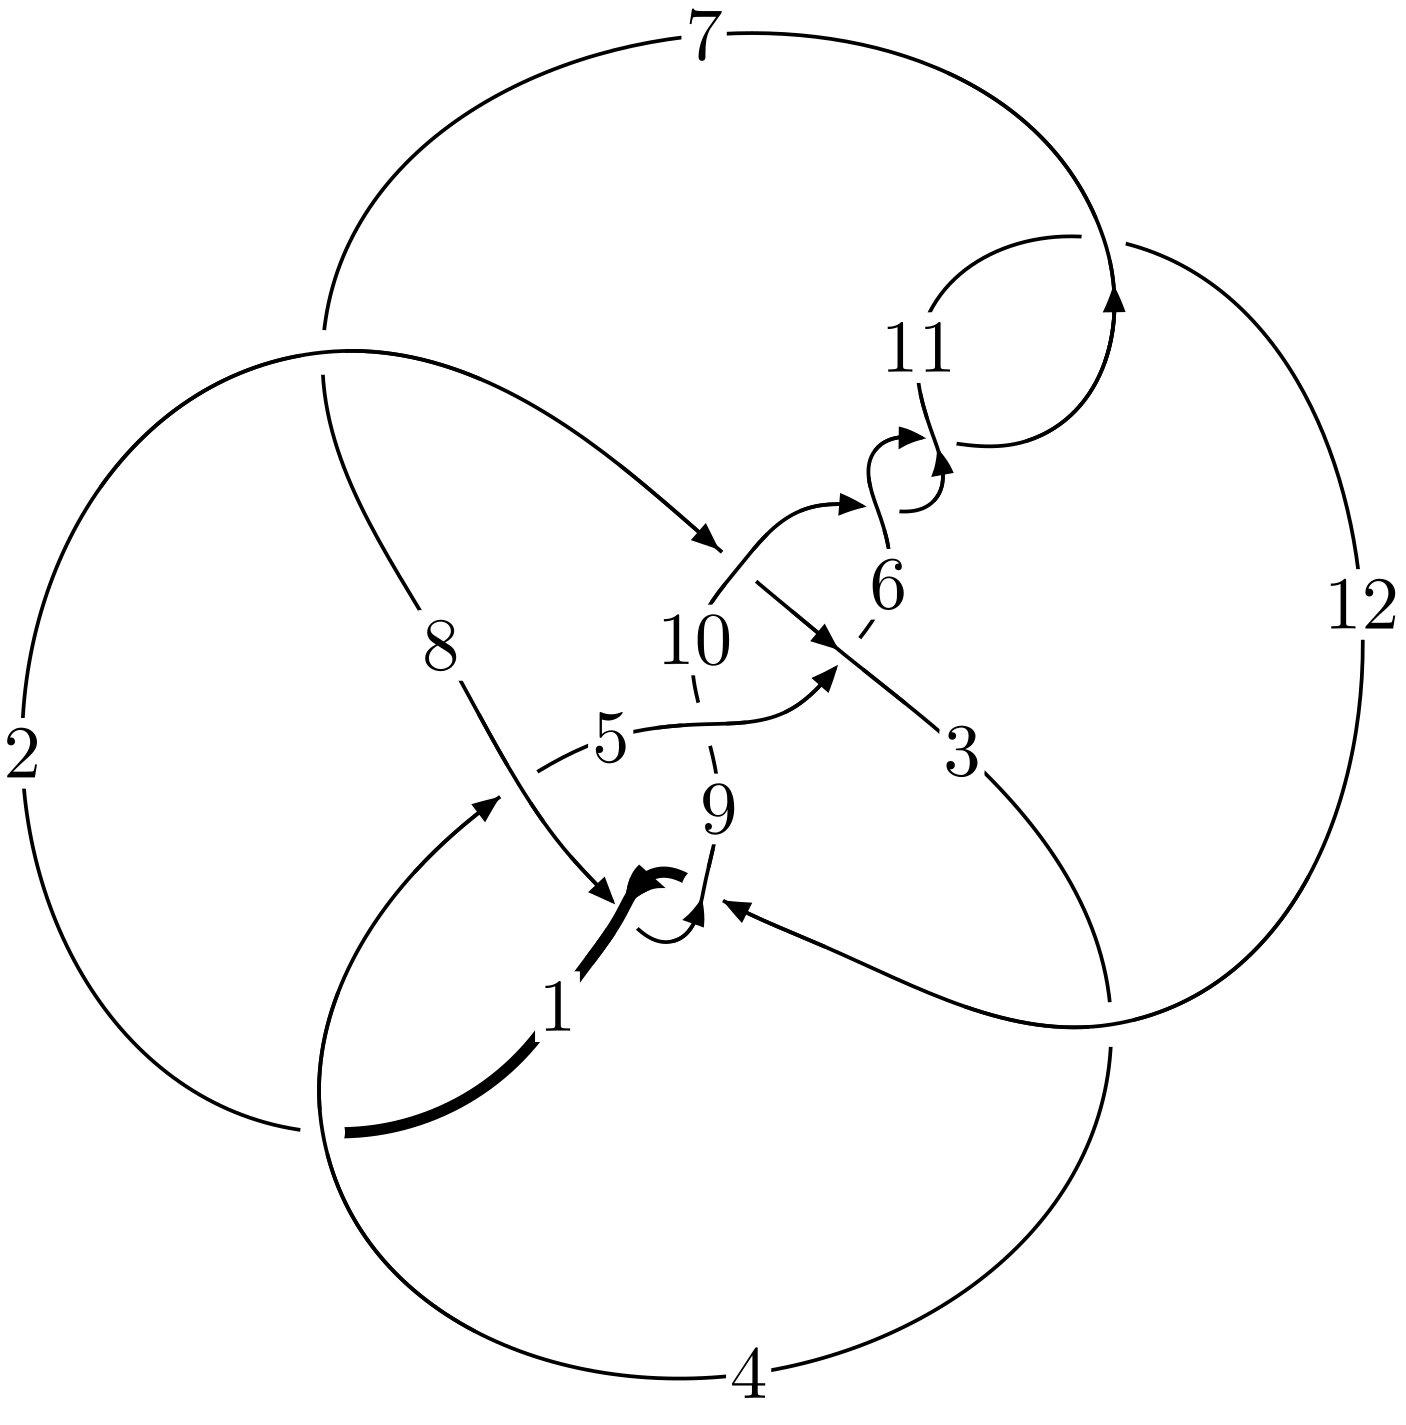
\includegraphics[width=112pt]{../../../GIT/diagram.site/Diagrams/png/1998_12a_1197.png}\\
\ \ \ A knot diagram\footnotemark}&
\allowdisplaybreaks
\textbf{Linearized knot diagam} \\
\cline{2-2}
 &
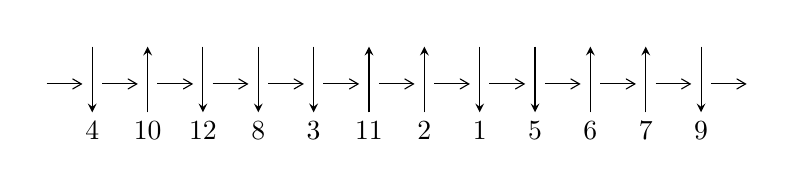
\begin{tikzpicture}[x=20pt, y=17pt]
	% nodes
	\node (C0) at (0, 0) {};
	\node (C1) at (1, 0) {};
	\node (C1U) at (1, +1) {};
	\node (C1D) at (1, -1) {4};

	\node (C2) at (2, 0) {};
	\node (C2U) at (2, +1) {};
	\node (C2D) at (2, -1) {10};

	\node (C3) at (3, 0) {};
	\node (C3U) at (3, +1) {};
	\node (C3D) at (3, -1) {12};

	\node (C4) at (4, 0) {};
	\node (C4U) at (4, +1) {};
	\node (C4D) at (4, -1) {8};

	\node (C5) at (5, 0) {};
	\node (C5U) at (5, +1) {};
	\node (C5D) at (5, -1) {3};

	\node (C6) at (6, 0) {};
	\node (C6U) at (6, +1) {};
	\node (C6D) at (6, -1) {11};

	\node (C7) at (7, 0) {};
	\node (C7U) at (7, +1) {};
	\node (C7D) at (7, -1) {2};

	\node (C8) at (8, 0) {};
	\node (C8U) at (8, +1) {};
	\node (C8D) at (8, -1) {1};

	\node (C9) at (9, 0) {};
	\node (C9U) at (9, +1) {};
	\node (C9D) at (9, -1) {5};

	\node (C10) at (10, 0) {};
	\node (C10U) at (10, +1) {};
	\node (C10D) at (10, -1) {6};

	\node (C11) at (11, 0) {};
	\node (C11U) at (11, +1) {};
	\node (C11D) at (11, -1) {7};

	\node (C12) at (12, 0) {};
	\node (C12U) at (12, +1) {};
	\node (C12D) at (12, -1) {9};
	\node (C13) at (13, 0) {};

	% arrows
	\draw[->,>={angle 60}]
	(C0) edge (C1) (C1) edge (C2) (C2) edge (C3) (C3) edge (C4) (C4) edge (C5) (C5) edge (C6) (C6) edge (C7) (C7) edge (C8) (C8) edge (C9) (C9) edge (C10) (C10) edge (C11) (C11) edge (C12) (C12) edge (C13) ;	\draw[->,>=stealth]
	(C1U) edge (C1D) (C2D) edge (C2U) (C3U) edge (C3D) (C4U) edge (C4D) (C5U) edge (C5D) (C6D) edge (C6U) (C7D) edge (C7U) (C8U) edge (C8D) (C9U) edge (C9D) (C10D) edge (C10U) (C11D) edge (C11U) (C12U) edge (C12D) ;
	\end{tikzpicture} \\
\hhline{~~} \\& 
\textbf{Solving Sequence} \\ \cline{2-2} 
 &
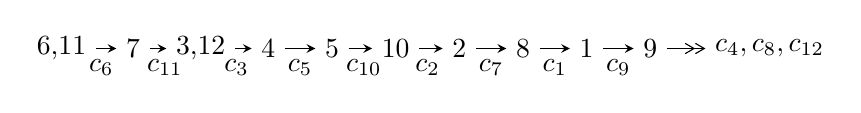
\begin{tikzpicture}[x=23pt, y=7pt]
	% node
	\node (A0) at (-1/8, 0) {6,11};
	\node (A1) at (1, 0) {7};
	\node (A2) at (33/16, 0) {3,12};
	\node (A3) at (25/8, 0) {4};
	\node (A4) at (33/8, 0) {5};
	\node (A5) at (41/8, 0) {10};
	\node (A6) at (49/8, 0) {2};
	\node (A7) at (57/8, 0) {8};
	\node (A8) at (65/8, 0) {1};
	\node (A9) at (73/8, 0) {9};
	\node (C1) at (1/2, -1) {$c_{6}$};
	\node (C2) at (3/2, -1) {$c_{11}$};
	\node (C3) at (21/8, -1) {$c_{3}$};
	\node (C4) at (29/8, -1) {$c_{5}$};
	\node (C5) at (37/8, -1) {$c_{10}$};
	\node (C6) at (45/8, -1) {$c_{2}$};
	\node (C7) at (53/8, -1) {$c_{7}$};
	\node (C8) at (61/8, -1) {$c_{1}$};
	\node (C9) at (69/8, -1) {$c_{9}$};
	\node (A10) at (11, 0) {$c_{4},c_{8},c_{12}$};

	% edge
	\draw[->,>=stealth]	
	(A0) edge (A1) (A1) edge (A2) (A2) edge (A3) (A3) edge (A4) (A4) edge (A5) (A5) edge (A6) (A6) edge (A7) (A7) edge (A8) (A8) edge (A9) ;
	\draw[->>,>={angle 60}]	
	(A9) edge (A10);
\end{tikzpicture} \\ 

\end{tabular} \\

\footnotetext{
The image of knot diagram is generated by the software ``\textbf{Draw programme}" developed by Andrew Bartholomew(\url{http://www.layer8.co.uk/maths/draw/index.htm\#Running-draw}), where we modified some parts for our purpose(\url{https://github.com/CATsTAILs/LinksPainter}).
}\phantom \\ \newline 
\centering \textbf{Ideals for irreducible components\footnotemark of $X_{\text{par}}$} 
 
\begin{align*}
I^u_{1}&=\langle 
-1.93169\times10^{465} u^{150}+6.15703\times10^{464} u^{149}+\cdots+1.03741\times10^{462} b-1.46910\times10^{465},\\
\phantom{I^u_{1}}&\phantom{= \langle  }2.56491\times10^{465} u^{150}-8.12627\times10^{464} u^{149}+\cdots+1.03741\times10^{462} a+2.03425\times10^{465},\;u^{151}+u^{150}+\cdots+32 u+1\rangle \\
I^u_{2}&=\langle 
-7692162316330 u^{29}+11057540047927 u^{28}+\cdots+19577401712437 b-8087783676063,\\
\phantom{I^u_{2}}&\phantom{= \langle  }46327339192051 u^{29}-8910173226523 u^{28}+\cdots+19577401712437 a+35928041395928,\\
\phantom{I^u_{2}}&\phantom{= \langle  }u^{30}- u^{29}+\cdots+3 u^2+1\rangle \\
I^u_{3}&=\langle 
b+1,\;a^3-2 a^2+a+1,\;u+1\rangle \\
\\
\end{align*}
\raggedright * 3 irreducible components of $\dim_{\mathbb{C}}=0$, with total 184 representations.\\
\footnotetext{All coefficients of polynomials are rational numbers. But the coefficients are sometimes approximated in decimal forms when there is not enough margin.}
\newpage
\renewcommand{\arraystretch}{1}
\centering \section*{I. $I^u_{1}= \langle -1.93\times10^{465} u^{150}+6.16\times10^{464} u^{149}+\cdots+1.04\times10^{462} b-1.47\times10^{465},\;2.56\times10^{465} u^{150}-8.13\times10^{464} u^{149}+\cdots+1.04\times10^{462} a+2.03\times10^{465},\;u^{151}+u^{150}+\cdots+32 u+1 \rangle$}
\flushleft \textbf{(i) Arc colorings}\\
\begin{tabular}{m{7pt} m{180pt} m{7pt} m{180pt} }
\flushright $a_{6}=$&$\begin{pmatrix}1\\0\end{pmatrix}$ \\
\flushright $a_{11}=$&$\begin{pmatrix}0\\u\end{pmatrix}$ \\
\flushright $a_{7}=$&$\begin{pmatrix}1\\- u^2\end{pmatrix}$ \\
\flushright $a_{3}=$&$\begin{pmatrix}-2472.41 u^{150}+783.321 u^{149}+\cdots-60019.0 u-1960.89\\1862.03 u^{150}-593.499 u^{149}+\cdots+44184.5 u+1416.12\end{pmatrix}$ \\
\flushright $a_{12}=$&$\begin{pmatrix}u\\- u^3+u\end{pmatrix}$ \\
\flushright $a_{4}=$&$\begin{pmatrix}-2525.32 u^{150}+798.167 u^{149}+\cdots-61301.5 u-2002.14\\1896.33 u^{150}-603.365 u^{149}+\cdots+45017.4 u+1442.63\end{pmatrix}$ \\
\flushright $a_{5}=$&$\begin{pmatrix}-1243.19 u^{150}+402.943 u^{149}+\cdots-28715.3 u-917.733\\1474.28 u^{150}-472.125 u^{149}+\cdots+34978.6 u+1121.68\end{pmatrix}$ \\
\flushright $a_{10}=$&$\begin{pmatrix}- u\\u\end{pmatrix}$ \\
\flushright $a_{2}=$&$\begin{pmatrix}-1414.94 u^{150}+443.487 u^{149}+\cdots-35022.8 u-1160.69\\804.555 u^{150}-253.665 u^{149}+\cdots+19188.2 u+615.911\end{pmatrix}$ \\
\flushright $a_{8}=$&$\begin{pmatrix}1246.81 u^{150}-395.426 u^{149}+\cdots+29898.5 u+949.873\\-1586.95 u^{150}+506.441 u^{149}+\cdots-37478.5 u-1197.23\end{pmatrix}$ \\
\flushright $a_{1}=$&$\begin{pmatrix}1468.40 u^{150}-478.505 u^{149}+\cdots+33223.5 u+1016.63\\-1479.74 u^{150}+476.894 u^{149}+\cdots-34849.1 u-1112.88\end{pmatrix}$ \\
\flushright $a_{9}=$&$\begin{pmatrix}410.152 u^{150}-117.692 u^{149}+\cdots+11541.2 u+398.278\\30.8075 u^{150}-12.2755 u^{149}+\cdots+664.532 u+22.0427\end{pmatrix}$\\&\end{tabular}
\flushleft \textbf{(ii) Obstruction class $= -1$}\\~\\
\flushleft \textbf{(iii) Cusp Shapes $= -1069.34 u^{150}+329.332 u^{149}+\cdots-25627.6 u-819.257$}\\~\\
\newpage\renewcommand{\arraystretch}{1}
\flushleft \textbf{(iv) u-Polynomials at the component}\newline \\
\begin{tabular}{m{50pt}|m{274pt}}
Crossings & \hspace{64pt}u-Polynomials at each crossing \\
\hline $$\begin{aligned}c_{1}\end{aligned}$$&$\begin{aligned}
&u^{151}+10 u^{150}+\cdots-31 u+23
\end{aligned}$\\
\hline $$\begin{aligned}c_{2}\end{aligned}$$&$\begin{aligned}
&u^{151}+3 u^{150}+\cdots+17222 u+2203
\end{aligned}$\\
\hline $$\begin{aligned}c_{3}\end{aligned}$$&$\begin{aligned}
&u^{151}-3 u^{150}+\cdots-514125 u+116356
\end{aligned}$\\
\hline $$\begin{aligned}c_{4}\end{aligned}$$&$\begin{aligned}
&u^{151}- u^{150}+\cdots+64 u+16
\end{aligned}$\\
\hline $$\begin{aligned}c_{5}\end{aligned}$$&$\begin{aligned}
&u^{151}+9 u^{150}+\cdots-6313 u+9724
\end{aligned}$\\
\hline $$\begin{aligned}c_{6},c_{10},c_{11}\end{aligned}$$&$\begin{aligned}
&u^{151}+u^{150}+\cdots+32 u+1
\end{aligned}$\\
\hline $$\begin{aligned}c_{7}\end{aligned}$$&$\begin{aligned}
&u^{151}-4 u^{150}+\cdots-2579090 u+234743
\end{aligned}$\\
\hline $$\begin{aligned}c_{8},c_{12}\end{aligned}$$&$\begin{aligned}
&u^{151}-2 u^{150}+\cdots+4057 u+1279
\end{aligned}$\\
\hline $$\begin{aligned}c_{9}\end{aligned}$$&$\begin{aligned}
&u^{151}-2 u^{150}+\cdots+492840 u+167911
\end{aligned}$\\
\hline
\end{tabular}\\~\\
\newpage\renewcommand{\arraystretch}{1}
\flushleft \textbf{(v) Riley Polynomials at the component}\newline \\
\begin{tabular}{m{50pt}|m{274pt}}
Crossings & \hspace{64pt}Riley Polynomials at each crossing \\
\hline $$\begin{aligned}c_{1}\end{aligned}$$&$\begin{aligned}
&y^{151}+18 y^{150}+\cdots-28249 y-529
\end{aligned}$\\
\hline $$\begin{aligned}c_{2}\end{aligned}$$&$\begin{aligned}
&y^{151}-13 y^{150}+\cdots+173229284 y-4853209
\end{aligned}$\\
\hline $$\begin{aligned}c_{3}\end{aligned}$$&$\begin{aligned}
&y^{151}-21 y^{150}+\cdots-752670674231 y-13538718736
\end{aligned}$\\
\hline $$\begin{aligned}c_{4}\end{aligned}$$&$\begin{aligned}
&y^{151}+y^{150}+\cdots-11136 y-256
\end{aligned}$\\
\hline $$\begin{aligned}c_{5}\end{aligned}$$&$\begin{aligned}
&y^{151}+21 y^{150}+\cdots-6011235647 y-94556176
\end{aligned}$\\
\hline $$\begin{aligned}c_{6},c_{10},c_{11}\end{aligned}$$&$\begin{aligned}
&y^{151}-149 y^{150}+\cdots+246 y-1
\end{aligned}$\\
\hline $$\begin{aligned}c_{7}\end{aligned}$$&$\begin{aligned}
&y^{151}+46 y^{150}+\cdots-7705800129308 y-55104276049
\end{aligned}$\\
\hline $$\begin{aligned}c_{8},c_{12}\end{aligned}$$&$\begin{aligned}
&y^{151}+94 y^{150}+\cdots-113123915 y-1635841
\end{aligned}$\\
\hline $$\begin{aligned}c_{9}\end{aligned}$$&$\begin{aligned}
&y^{151}-56 y^{150}+\cdots+725298561134 y-28194103921
\end{aligned}$\\
\hline
\end{tabular}\\~\\
\newpage\flushleft \textbf{(vi) Complex Volumes and Cusp Shapes}
$$\begin{array}{c|c|c}  
\text{Solutions to }I^u_{1}& \I (\text{vol} + \sqrt{-1}CS) & \text{Cusp shape}\\
 \hline 
\begin{aligned}
u &= \phantom{-}0.472050 + 0.884004 I \\
a &= -0.066559 - 0.608220 I \\
b &= -0.865778 + 0.742016 I\end{aligned}
 & -1.71499 + 3.44862 I & \phantom{-0.000000 } 0 \\ \hline\begin{aligned}
u &= \phantom{-}0.472050 - 0.884004 I \\
a &= -0.066559 + 0.608220 I \\
b &= -0.865778 - 0.742016 I\end{aligned}
 & -1.71499 - 3.44862 I & \phantom{-0.000000 } 0 \\ \hline\begin{aligned}
u &= \phantom{-}0.504245 + 0.856993 I \\
a &= \phantom{-}0.408980 + 0.667727 I \\
b &= \phantom{-}0.95994 - 1.03916 I\end{aligned}
 & \phantom{-}0.0365 + 15.6382 I & \phantom{-0.000000 } 0 \\ \hline\begin{aligned}
u &= \phantom{-}0.504245 - 0.856993 I \\
a &= \phantom{-}0.408980 - 0.667727 I \\
b &= \phantom{-}0.95994 + 1.03916 I\end{aligned}
 & \phantom{-}0.0365 - 15.6382 I & \phantom{-0.000000 } 0 \\ \hline\begin{aligned}
u &= \phantom{-}0.912866 + 0.388375 I \\
a &= \phantom{-}1.180150 - 0.056109 I \\
b &= -0.704000 - 0.782081 I\end{aligned}
 & \phantom{-}1.12038 - 2.21817 I & \phantom{-0.000000 } 0 \\ \hline\begin{aligned}
u &= \phantom{-}0.912866 - 0.388375 I \\
a &= \phantom{-}1.180150 + 0.056109 I \\
b &= -0.704000 + 0.782081 I\end{aligned}
 & \phantom{-}1.12038 + 2.21817 I & \phantom{-0.000000 } 0 \\ \hline\begin{aligned}
u &= -0.611081 + 0.775672 I \\
a &= -0.266528 + 1.168600 I \\
b &= -0.938329 - 1.024730 I\end{aligned}
 & -1.20004 - 5.85292 I & \phantom{-0.000000 } 0 \\ \hline\begin{aligned}
u &= -0.611081 - 0.775672 I \\
a &= -0.266528 - 1.168600 I \\
b &= -0.938329 + 1.024730 I\end{aligned}
 & -1.20004 + 5.85292 I & \phantom{-0.000000 } 0 \\ \hline\begin{aligned}
u &= -0.503327 + 0.841973 I \\
a &= \phantom{-}0.405727 - 0.542238 I \\
b &= \phantom{-}0.940020 + 0.870651 I\end{aligned}
 & -3.87850 - 9.51725 I & \phantom{-0.000000 } 0 \\ \hline\begin{aligned}
u &= -0.503327 - 0.841973 I \\
a &= \phantom{-}0.405727 + 0.542238 I \\
b &= \phantom{-}0.940020 - 0.870651 I\end{aligned}
 & -3.87850 + 9.51725 I & \phantom{-0.000000 } 0\\
 \hline 
 \end{array}$$\newpage$$\begin{array}{c|c|c}  
\text{Solutions to }I^u_{1}& \I (\text{vol} + \sqrt{-1}CS) & \text{Cusp shape}\\
 \hline 
\begin{aligned}
u &= -1.006270 + 0.228464 I \\
a &= \phantom{-}1.216270 + 0.711644 I \\
b &= -0.847046 + 0.388872 I\end{aligned}
 & -0.037294 + 1.011850 I & \phantom{-0.000000 } 0 \\ \hline\begin{aligned}
u &= -1.006270 - 0.228464 I \\
a &= \phantom{-}1.216270 - 0.711644 I \\
b &= -0.847046 - 0.388872 I\end{aligned}
 & -0.037294 - 1.011850 I & \phantom{-0.000000 } 0 \\ \hline\begin{aligned}
u &= \phantom{-}0.307987 + 1.007600 I \\
a &= \phantom{-}0.0145948 - 0.0417020 I \\
b &= -0.243767 + 0.424475 I\end{aligned}
 & -0.97150 + 2.88010 I & \phantom{-0.000000 } 0 \\ \hline\begin{aligned}
u &= \phantom{-}0.307987 - 1.007600 I \\
a &= \phantom{-}0.0145948 + 0.0417020 I \\
b &= -0.243767 - 0.424475 I\end{aligned}
 & -0.97150 - 2.88010 I & \phantom{-0.000000 } 0 \\ \hline\begin{aligned}
u &= \phantom{-}0.451480 + 0.831454 I \\
a &= \phantom{-}0.679184 + 0.277402 I \\
b &= \phantom{-}0.551251 - 0.635164 I\end{aligned}
 & \phantom{-}2.01542 + 3.29869 I & \phantom{-0.000000 } 0 \\ \hline\begin{aligned}
u &= \phantom{-}0.451480 - 0.831454 I \\
a &= \phantom{-}0.679184 - 0.277402 I \\
b &= \phantom{-}0.551251 + 0.635164 I\end{aligned}
 & \phantom{-}2.01542 - 3.29869 I & \phantom{-0.000000 } 0 \\ \hline\begin{aligned}
u &= \phantom{-}0.662919 + 0.657611 I \\
a &= -0.019360 - 0.205176 I \\
b &= -0.041555 + 0.763269 I\end{aligned}
 & \phantom{-}2.82346 + 1.75052 I & \phantom{-0.000000 } 0 \\ \hline\begin{aligned}
u &= \phantom{-}0.662919 - 0.657611 I \\
a &= -0.019360 + 0.205176 I \\
b &= -0.041555 - 0.763269 I\end{aligned}
 & \phantom{-}2.82346 - 1.75052 I & \phantom{-0.000000 } 0 \\ \hline\begin{aligned}
u &= -0.289908 + 0.878176 I \\
a &= -0.403446 + 0.003942 I \\
b &= -0.111239 - 1.043220 I\end{aligned}
 & \phantom{-}4.09674 - 6.13896 I & \phantom{-0.000000 } 0 \\ \hline\begin{aligned}
u &= -0.289908 - 0.878176 I \\
a &= -0.403446 - 0.003942 I \\
b &= -0.111239 + 1.043220 I\end{aligned}
 & \phantom{-}4.09674 + 6.13896 I & \phantom{-0.000000 } 0\\
 \hline 
 \end{array}$$\newpage$$\begin{array}{c|c|c}  
\text{Solutions to }I^u_{1}& \I (\text{vol} + \sqrt{-1}CS) & \text{Cusp shape}\\
 \hline 
\begin{aligned}
u &= -0.680650 + 0.853136 I \\
a &= -0.404161 - 0.241544 I \\
b &= \phantom{-}0.556428 - 0.537921 I\end{aligned}
 & -3.44023 + 3.92803 I & \phantom{-0.000000 } 0 \\ \hline\begin{aligned}
u &= -0.680650 - 0.853136 I \\
a &= -0.404161 + 0.241544 I \\
b &= \phantom{-}0.556428 + 0.537921 I\end{aligned}
 & -3.44023 - 3.92803 I & \phantom{-0.000000 } 0 \\ \hline\begin{aligned}
u &= \phantom{-}0.692681 + 0.848382 I \\
a &= -0.601898 + 0.126360 I \\
b &= \phantom{-}0.661284 + 0.730649 I\end{aligned}
 & \phantom{-}0.52013 - 9.98699 I & \phantom{-0.000000 } 0 \\ \hline\begin{aligned}
u &= \phantom{-}0.692681 - 0.848382 I \\
a &= -0.601898 - 0.126360 I \\
b &= \phantom{-}0.661284 - 0.730649 I\end{aligned}
 & \phantom{-}0.52013 + 9.98699 I & \phantom{-0.000000 } 0 \\ \hline\begin{aligned}
u &= -0.719832 + 0.492448 I \\
a &= \phantom{-}1.399660 - 0.089298 I \\
b &= -0.547746 + 0.373026 I\end{aligned}
 & \phantom{-}1.12644 - 1.02234 I & \phantom{-0.000000 } 0 \\ \hline\begin{aligned}
u &= -0.719832 - 0.492448 I \\
a &= \phantom{-}1.399660 + 0.089298 I \\
b &= -0.547746 - 0.373026 I\end{aligned}
 & \phantom{-}1.12644 + 1.02234 I & \phantom{-0.000000 } 0 \\ \hline\begin{aligned}
u &= \phantom{-}1.16581\phantom{ +0.000000I} \\
a &= \phantom{-}0.625214\phantom{ +0.000000I} \\
b &= \phantom{-}0.958492\phantom{ +0.000000I}\end{aligned}
 & -0.203933\phantom{ +0.000000I} & \phantom{-0.000000 } 0 \\ \hline\begin{aligned}
u &= -0.088671 + 0.819822 I \\
a &= \phantom{-}0.178460 - 0.665085 I \\
b &= \phantom{-}0.501925 - 0.506145 I\end{aligned}
 & \phantom{-}1.03243 + 3.95432 I & \phantom{-0.000000 } 0 \\ \hline\begin{aligned}
u &= -0.088671 - 0.819822 I \\
a &= \phantom{-}0.178460 + 0.665085 I \\
b &= \phantom{-}0.501925 + 0.506145 I\end{aligned}
 & \phantom{-}1.03243 - 3.95432 I & \phantom{-0.000000 } 0 \\ \hline\begin{aligned}
u &= \phantom{-}0.294379 + 0.769396 I \\
a &= -0.566559 - 0.276220 I \\
b &= -0.89715 + 1.15300 I\end{aligned}
 & -0.74749 + 6.51000 I & \phantom{-0.000000 } 0\\
 \hline 
 \end{array}$$\newpage$$\begin{array}{c|c|c}  
\text{Solutions to }I^u_{1}& \I (\text{vol} + \sqrt{-1}CS) & \text{Cusp shape}\\
 \hline 
\begin{aligned}
u &= \phantom{-}0.294379 - 0.769396 I \\
a &= -0.566559 + 0.276220 I \\
b &= -0.89715 - 1.15300 I\end{aligned}
 & -0.74749 - 6.51000 I & \phantom{-0.000000 } 0 \\ \hline\begin{aligned}
u &= \phantom{-}1.18028\phantom{ +0.000000I} \\
a &= \phantom{-}0.639260\phantom{ +0.000000I} \\
b &= \phantom{-}0.954322\phantom{ +0.000000I}\end{aligned}
 & -0.203875\phantom{ +0.000000I} & \phantom{-0.000000 } 0 \\ \hline\begin{aligned}
u &= \phantom{-}0.767722 + 0.269242 I \\
a &= -0.94336 - 2.30227 I \\
b &= -0.251496 + 1.103530 I\end{aligned}
 & \phantom{-}2.38552 + 6.45222 I & \phantom{-0.000000 } 0 \\ \hline\begin{aligned}
u &= \phantom{-}0.767722 - 0.269242 I \\
a &= -0.94336 + 2.30227 I \\
b &= -0.251496 - 1.103530 I\end{aligned}
 & \phantom{-}2.38552 - 6.45222 I & \phantom{-0.000000 } 0 \\ \hline\begin{aligned}
u &= \phantom{-}1.194630 + 0.039800 I \\
a &= -0.30353 - 2.67611 I \\
b &= \phantom{-}0.00986 + 1.76611 I\end{aligned}
 & \phantom{-}2.58122 + 6.21762 I & \phantom{-0.000000 } 0 \\ \hline\begin{aligned}
u &= \phantom{-}1.194630 - 0.039800 I \\
a &= -0.30353 + 2.67611 I \\
b &= \phantom{-}0.00986 - 1.76611 I\end{aligned}
 & \phantom{-}2.58122 - 6.21762 I & \phantom{-0.000000 } 0 \\ \hline\begin{aligned}
u &= -0.666938 + 0.432809 I \\
a &= \phantom{-}0.857628 - 0.684938 I \\
b &= \phantom{-}0.333070 + 1.027970 I\end{aligned}
 & \phantom{-}5.90452 + 1.69142 I & \phantom{-0.000000 } 0 \\ \hline\begin{aligned}
u &= -0.666938 - 0.432809 I \\
a &= \phantom{-}0.857628 + 0.684938 I \\
b &= \phantom{-}0.333070 - 1.027970 I\end{aligned}
 & \phantom{-}5.90452 - 1.69142 I & \phantom{-0.000000 } 0 \\ \hline\begin{aligned}
u &= \phantom{-}0.466756 + 0.642700 I \\
a &= \phantom{-}0.316550 + 0.923918 I \\
b &= \phantom{-}0.512069 - 0.068322 I\end{aligned}
 & \phantom{-}0.36618 + 2.92618 I & \phantom{-0.000000 } 0 \\ \hline\begin{aligned}
u &= \phantom{-}0.466756 - 0.642700 I \\
a &= \phantom{-}0.316550 - 0.923918 I \\
b &= \phantom{-}0.512069 + 0.068322 I\end{aligned}
 & \phantom{-}0.36618 - 2.92618 I & \phantom{-0.000000 } 0\\
 \hline 
 \end{array}$$\newpage$$\begin{array}{c|c|c}  
\text{Solutions to }I^u_{1}& \I (\text{vol} + \sqrt{-1}CS) & \text{Cusp shape}\\
 \hline 
\begin{aligned}
u &= \phantom{-}0.576637 + 0.541410 I \\
a &= \phantom{-}0.469384 + 0.295539 I \\
b &= \phantom{-}0.830869 - 0.401613 I\end{aligned}
 & \phantom{-}0.83324 + 1.17258 I & \phantom{-0.000000 } 0 \\ \hline\begin{aligned}
u &= \phantom{-}0.576637 - 0.541410 I \\
a &= \phantom{-}0.469384 - 0.295539 I \\
b &= \phantom{-}0.830869 + 0.401613 I\end{aligned}
 & \phantom{-}0.83324 - 1.17258 I & \phantom{-0.000000 } 0 \\ \hline\begin{aligned}
u &= \phantom{-}0.726822 + 0.968082 I \\
a &= \phantom{-}0.357375 + 0.005289 I \\
b &= -0.485392 - 0.257705 I\end{aligned}
 & -1.11296 + 2.52087 I & \phantom{-0.000000 } 0 \\ \hline\begin{aligned}
u &= \phantom{-}0.726822 - 0.968082 I \\
a &= \phantom{-}0.357375 - 0.005289 I \\
b &= -0.485392 + 0.257705 I\end{aligned}
 & -1.11296 - 2.52087 I & \phantom{-0.000000 } 0 \\ \hline\begin{aligned}
u &= \phantom{-}0.771651 + 0.143074 I \\
a &= \phantom{-}1.348220 - 0.330576 I \\
b &= -0.659980 + 0.317289 I\end{aligned}
 & \phantom{-}1.47481 + 1.99247 I & \phantom{-0.000000 } 0 \\ \hline\begin{aligned}
u &= \phantom{-}0.771651 - 0.143074 I \\
a &= \phantom{-}1.348220 + 0.330576 I \\
b &= -0.659980 - 0.317289 I\end{aligned}
 & \phantom{-}1.47481 - 1.99247 I & \phantom{-0.000000 } 0 \\ \hline\begin{aligned}
u &= \phantom{-}1.251800 + 0.039923 I \\
a &= \phantom{-}1.47364 - 0.18892 I \\
b &= -1.56675 + 0.30763 I\end{aligned}
 & \phantom{-}1.83875 + 1.81155 I & \phantom{-0.000000 } 0 \\ \hline\begin{aligned}
u &= \phantom{-}1.251800 - 0.039923 I \\
a &= \phantom{-}1.47364 + 0.18892 I \\
b &= -1.56675 - 0.30763 I\end{aligned}
 & \phantom{-}1.83875 - 1.81155 I & \phantom{-0.000000 } 0 \\ \hline\begin{aligned}
u &= -0.606001 + 0.422787 I \\
a &= \phantom{-}0.297448 - 0.682730 I \\
b &= \phantom{-}1.12975 + 0.89007 I\end{aligned}
 & \phantom{-}2.97652 - 7.77376 I & \phantom{-0.000000 } 0 \\ \hline\begin{aligned}
u &= -0.606001 - 0.422787 I \\
a &= \phantom{-}0.297448 + 0.682730 I \\
b &= \phantom{-}1.12975 - 0.89007 I\end{aligned}
 & \phantom{-}2.97652 + 7.77376 I & \phantom{-0.000000 } 0\\
 \hline 
 \end{array}$$\newpage$$\begin{array}{c|c|c}  
\text{Solutions to }I^u_{1}& \I (\text{vol} + \sqrt{-1}CS) & \text{Cusp shape}\\
 \hline 
\begin{aligned}
u &= -1.266550 + 0.008705 I \\
a &= \phantom{-}0.556477 - 0.495290 I \\
b &= \phantom{-}1.000120 + 0.422333 I\end{aligned}
 & \phantom{-}3.57413 - 6.67964 I & \phantom{-0.000000 } 0 \\ \hline\begin{aligned}
u &= -1.266550 - 0.008705 I \\
a &= \phantom{-}0.556477 + 0.495290 I \\
b &= \phantom{-}1.000120 - 0.422333 I\end{aligned}
 & \phantom{-}3.57413 + 6.67964 I & \phantom{-0.000000 } 0 \\ \hline\begin{aligned}
u &= -0.099423 + 0.717248 I \\
a &= \phantom{-}0.088176 + 0.562484 I \\
b &= -0.847484 - 1.026340 I\end{aligned}
 & -0.81884 - 2.99177 I & \phantom{-0.000000 } 0 \\ \hline\begin{aligned}
u &= -0.099423 - 0.717248 I \\
a &= \phantom{-}0.088176 - 0.562484 I \\
b &= -0.847484 + 1.026340 I\end{aligned}
 & -0.81884 + 2.99177 I & \phantom{-0.000000 } 0 \\ \hline\begin{aligned}
u &= -1.275840 + 0.028854 I \\
a &= \phantom{-}1.51296 + 0.05179 I \\
b &= -1.90289 + 0.18009 I\end{aligned}
 & \phantom{-}1.19324 - 0.84761 I & \phantom{-0.000000 } 0 \\ \hline\begin{aligned}
u &= -1.275840 - 0.028854 I \\
a &= \phantom{-}1.51296 - 0.05179 I \\
b &= -1.90289 - 0.18009 I\end{aligned}
 & \phantom{-}1.19324 + 0.84761 I & \phantom{-0.000000 } 0 \\ \hline\begin{aligned}
u &= -0.374955 + 0.586656 I \\
a &= \phantom{-}0.328445 + 0.196934 I \\
b &= -0.796211 + 0.663794 I\end{aligned}
 & -1.92772 + 0.99887 I & \phantom{-0.000000 } 0 \\ \hline\begin{aligned}
u &= -0.374955 - 0.586656 I \\
a &= \phantom{-}0.328445 - 0.196934 I \\
b &= -0.796211 - 0.663794 I\end{aligned}
 & -1.92772 - 0.99887 I & \phantom{-0.000000 } 0 \\ \hline\begin{aligned}
u &= -1.285530 + 0.224675 I \\
a &= \phantom{-}0.600454 - 0.994227 I \\
b &= \phantom{-}0.236056 + 1.049820 I\end{aligned}
 & \phantom{-}6.60594 + 2.14914 I & \phantom{-0.000000 } 0 \\ \hline\begin{aligned}
u &= -1.285530 - 0.224675 I \\
a &= \phantom{-}0.600454 + 0.994227 I \\
b &= \phantom{-}0.236056 - 1.049820 I\end{aligned}
 & \phantom{-}6.60594 - 2.14914 I & \phantom{-0.000000 } 0\\
 \hline 
 \end{array}$$\newpage$$\begin{array}{c|c|c}  
\text{Solutions to }I^u_{1}& \I (\text{vol} + \sqrt{-1}CS) & \text{Cusp shape}\\
 \hline 
\begin{aligned}
u &= -0.314366 + 0.611307 I \\
a &= -1.076990 + 0.329028 I \\
b &= -0.955686 - 0.827991 I\end{aligned}
 & -2.01575 - 4.12490 I & \phantom{-0.000000 } 0 \\ \hline\begin{aligned}
u &= -0.314366 - 0.611307 I \\
a &= -1.076990 - 0.329028 I \\
b &= -0.955686 + 0.827991 I\end{aligned}
 & -2.01575 + 4.12490 I & \phantom{-0.000000 } 0 \\ \hline\begin{aligned}
u &= \phantom{-}1.314370 + 0.054225 I \\
a &= \phantom{-}0.63928 - 1.81129 I \\
b &= -0.221124 + 0.619361 I\end{aligned}
 & \phantom{-}2.21104 + 1.53029 I & \phantom{-0.000000 } 0 \\ \hline\begin{aligned}
u &= \phantom{-}1.314370 - 0.054225 I \\
a &= \phantom{-}0.63928 + 1.81129 I \\
b &= -0.221124 - 0.619361 I\end{aligned}
 & \phantom{-}2.21104 - 1.53029 I & \phantom{-0.000000 } 0 \\ \hline\begin{aligned}
u &= -0.226306 + 0.644285 I \\
a &= \phantom{-}0.193572 + 0.017568 I \\
b &= -0.901110 + 0.749271 I\end{aligned}
 & -1.97131 + 0.98981 I & \phantom{-0.000000 } 0 \\ \hline\begin{aligned}
u &= -0.226306 - 0.644285 I \\
a &= \phantom{-}0.193572 - 0.017568 I \\
b &= -0.901110 - 0.749271 I\end{aligned}
 & -1.97131 - 0.98981 I & \phantom{-0.000000 } 0 \\ \hline\begin{aligned}
u &= -1.319580 + 0.000470 I \\
a &= \phantom{-}0.15449 + 2.89765 I \\
b &= -0.41715 - 2.16203 I\end{aligned}
 & \phantom{-}0.74888 - 2.07009 I & \phantom{-0.000000 } 0 \\ \hline\begin{aligned}
u &= -1.319580 - 0.000470 I \\
a &= \phantom{-}0.15449 - 2.89765 I \\
b &= -0.41715 + 2.16203 I\end{aligned}
 & \phantom{-}0.74888 + 2.07009 I & \phantom{-0.000000 } 0 \\ \hline\begin{aligned}
u &= -1.325950 + 0.072576 I \\
a &= -0.22273 - 2.02390 I \\
b &= \phantom{-}0.006077 + 0.210149 I\end{aligned}
 & \phantom{-}0.33089 - 3.72354 I & \phantom{-0.000000 } 0 \\ \hline\begin{aligned}
u &= -1.325950 - 0.072576 I \\
a &= -0.22273 + 2.02390 I \\
b &= \phantom{-}0.006077 - 0.210149 I\end{aligned}
 & \phantom{-}0.33089 + 3.72354 I & \phantom{-0.000000 } 0\\
 \hline 
 \end{array}$$\newpage$$\begin{array}{c|c|c}  
\text{Solutions to }I^u_{1}& \I (\text{vol} + \sqrt{-1}CS) & \text{Cusp shape}\\
 \hline 
\begin{aligned}
u &= \phantom{-}0.501132 + 0.424261 I \\
a &= \phantom{-}0.774921 + 0.176630 I \\
b &= \phantom{-}0.392521 - 0.225566 I\end{aligned}
 & \phantom{-}1.02977 + 1.08869 I & \phantom{-0.000000 } 0 \\ \hline\begin{aligned}
u &= \phantom{-}0.501132 - 0.424261 I \\
a &= \phantom{-}0.774921 - 0.176630 I \\
b &= \phantom{-}0.392521 + 0.225566 I\end{aligned}
 & \phantom{-}1.02977 - 1.08869 I & \phantom{-0.000000 } 0 \\ \hline\begin{aligned}
u &= \phantom{-}1.359840 + 0.106565 I \\
a &= \phantom{-}0.38150 - 2.26011 I \\
b &= -0.407501 + 1.332490 I\end{aligned}
 & \phantom{-}2.43991 + 2.33188 I & \phantom{-0.000000 } 0 \\ \hline\begin{aligned}
u &= \phantom{-}1.359840 - 0.106565 I \\
a &= \phantom{-}0.38150 + 2.26011 I \\
b &= -0.407501 - 1.332490 I\end{aligned}
 & \phantom{-}2.43991 - 2.33188 I & \phantom{-0.000000 } 0 \\ \hline\begin{aligned}
u &= -1.372460 + 0.115018 I \\
a &= -2.07479 + 0.74394 I \\
b &= \phantom{-}2.31167 - 0.86468 I\end{aligned}
 & \phantom{-}4.50244 - 9.81798 I & \phantom{-0.000000 } 0 \\ \hline\begin{aligned}
u &= -1.372460 - 0.115018 I \\
a &= -2.07479 - 0.74394 I \\
b &= \phantom{-}2.31167 + 0.86468 I\end{aligned}
 & \phantom{-}4.50244 + 9.81798 I & \phantom{-0.000000 } 0 \\ \hline\begin{aligned}
u &= -1.376410 + 0.053949 I \\
a &= \phantom{-}0.439738 - 0.430662 I \\
b &= -1.45268 + 0.38145 I\end{aligned}
 & \phantom{-}2.51893 - 0.80202 I & \phantom{-0.000000 } 0 \\ \hline\begin{aligned}
u &= -1.376410 - 0.053949 I \\
a &= \phantom{-}0.439738 + 0.430662 I \\
b &= -1.45268 - 0.38145 I\end{aligned}
 & \phantom{-}2.51893 + 0.80202 I & \phantom{-0.000000 } 0 \\ \hline\begin{aligned}
u &= \phantom{-}1.392990 + 0.092555 I \\
a &= -1.03769 + 2.11407 I \\
b &= \phantom{-}0.103443 - 0.346460 I\end{aligned}
 & \phantom{-}5.20516 + 9.30317 I & \phantom{-0.000000 } 0 \\ \hline\begin{aligned}
u &= \phantom{-}1.392990 - 0.092555 I \\
a &= -1.03769 - 2.11407 I \\
b &= \phantom{-}0.103443 + 0.346460 I\end{aligned}
 & \phantom{-}5.20516 - 9.30317 I & \phantom{-0.000000 } 0\\
 \hline 
 \end{array}$$\newpage$$\begin{array}{c|c|c}  
\text{Solutions to }I^u_{1}& \I (\text{vol} + \sqrt{-1}CS) & \text{Cusp shape}\\
 \hline 
\begin{aligned}
u &= -1.393310 + 0.092532 I \\
a &= \phantom{-}0.35300 + 2.65057 I \\
b &= -0.64454 - 1.55997 I\end{aligned}
 & \phantom{-}3.56985 - 4.53824 I & \phantom{-0.000000 } 0 \\ \hline\begin{aligned}
u &= -1.393310 - 0.092532 I \\
a &= \phantom{-}0.35300 - 2.65057 I \\
b &= -0.64454 + 1.55997 I\end{aligned}
 & \phantom{-}3.56985 + 4.53824 I & \phantom{-0.000000 } 0 \\ \hline\begin{aligned}
u &= \phantom{-}1.395620 + 0.092828 I \\
a &= -1.49502 - 1.58215 I \\
b &= \phantom{-}1.73103 + 1.54682 I\end{aligned}
 & \phantom{-}2.26519 + 4.19440 I & \phantom{-0.000000 } 0 \\ \hline\begin{aligned}
u &= \phantom{-}1.395620 - 0.092828 I \\
a &= -1.49502 + 1.58215 I \\
b &= \phantom{-}1.73103 - 1.54682 I\end{aligned}
 & \phantom{-}2.26519 - 4.19440 I & \phantom{-0.000000 } 0 \\ \hline\begin{aligned}
u &= \phantom{-}1.41149 + 0.12685 I \\
a &= -0.040753 - 1.036190 I \\
b &= -1.186810 + 0.482059 I\end{aligned}
 & \phantom{-}3.47980 + 5.91274 I & \phantom{-0.000000 } 0 \\ \hline\begin{aligned}
u &= \phantom{-}1.41149 - 0.12685 I \\
a &= -0.040753 + 1.036190 I \\
b &= -1.186810 - 0.482059 I\end{aligned}
 & \phantom{-}3.47980 - 5.91274 I & \phantom{-0.000000 } 0 \\ \hline\begin{aligned}
u &= \phantom{-}1.41753 + 0.01543 I \\
a &= -0.26012 + 1.98695 I \\
b &= -0.700504 - 1.140990 I\end{aligned}
 & \phantom{-}8.08358 - 2.80885 I & \phantom{-0.000000 } 0 \\ \hline\begin{aligned}
u &= \phantom{-}1.41753 - 0.01543 I \\
a &= -0.26012 - 1.98695 I \\
b &= -0.700504 + 1.140990 I\end{aligned}
 & \phantom{-}8.08358 + 2.80885 I & \phantom{-0.000000 } 0 \\ \hline\begin{aligned}
u &= \phantom{-}1.41337 + 0.32587 I \\
a &= \phantom{-}0.391511 + 0.900541 I \\
b &= \phantom{-}0.210075 - 0.759023 I\end{aligned}
 & \phantom{-}2.96910 + 1.89636 I & \phantom{-0.000000 } 0 \\ \hline\begin{aligned}
u &= \phantom{-}1.41337 - 0.32587 I \\
a &= \phantom{-}0.391511 - 0.900541 I \\
b &= \phantom{-}0.210075 + 0.759023 I\end{aligned}
 & \phantom{-}2.96910 - 1.89636 I & \phantom{-0.000000 } 0\\
 \hline 
 \end{array}$$\newpage$$\begin{array}{c|c|c}  
\text{Solutions to }I^u_{1}& \I (\text{vol} + \sqrt{-1}CS) & \text{Cusp shape}\\
 \hline 
\begin{aligned}
u &= -1.45986 + 0.04354 I \\
a &= \phantom{-}0.408620 + 0.933157 I \\
b &= \phantom{-}0.379155 - 0.667460 I\end{aligned}
 & \phantom{-}8.29942 - 2.47433 I & \phantom{-0.000000 } 0 \\ \hline\begin{aligned}
u &= -1.45986 - 0.04354 I \\
a &= \phantom{-}0.408620 - 0.933157 I \\
b &= \phantom{-}0.379155 + 0.667460 I\end{aligned}
 & \phantom{-}8.29942 + 2.47433 I & \phantom{-0.000000 } 0 \\ \hline\begin{aligned}
u &= \phantom{-}1.44853 + 0.23223 I \\
a &= \phantom{-}0.03102 - 1.82557 I \\
b &= -1.08265 + 1.19970 I\end{aligned}
 & \phantom{-}3.72729 + 7.23890 I & \phantom{-0.000000 } 0 \\ \hline\begin{aligned}
u &= \phantom{-}1.44853 - 0.23223 I \\
a &= \phantom{-}0.03102 + 1.82557 I \\
b &= -1.08265 - 1.19970 I\end{aligned}
 & \phantom{-}3.72729 - 7.23890 I & \phantom{-0.000000 } 0 \\ \hline\begin{aligned}
u &= -1.44057 + 0.29049 I \\
a &= -0.08711 + 1.97285 I \\
b &= -0.99032 - 1.49431 I\end{aligned}
 & \phantom{-}4.83658 - 10.34260 I & \phantom{-0.000000 } 0 \\ \hline\begin{aligned}
u &= -1.44057 - 0.29049 I \\
a &= -0.08711 - 1.97285 I \\
b &= -0.99032 + 1.49431 I\end{aligned}
 & \phantom{-}4.83658 + 10.34260 I & \phantom{-0.000000 } 0 \\ \hline\begin{aligned}
u &= -0.273659 + 0.438926 I \\
a &= -2.06869 + 0.18529 I \\
b &= -0.818659 - 0.523077 I\end{aligned}
 & -1.90487 - 3.92884 I & -7.58573 + 9.42654 I \\ \hline\begin{aligned}
u &= -0.273659 - 0.438926 I \\
a &= -2.06869 - 0.18529 I \\
b &= -0.818659 + 0.523077 I\end{aligned}
 & -1.90487 + 3.92884 I & -7.58573 - 9.42654 I \\ \hline\begin{aligned}
u &= -1.48690 + 0.16147 I \\
a &= -0.079299 - 0.792708 I \\
b &= \phantom{-}0.854653 + 0.548893 I\end{aligned}
 & \phantom{-}7.49359 - 3.32401 I & \phantom{-0.000000 } 0 \\ \hline\begin{aligned}
u &= -1.48690 - 0.16147 I \\
a &= -0.079299 + 0.792708 I \\
b &= \phantom{-}0.854653 - 0.548893 I\end{aligned}
 & \phantom{-}7.49359 + 3.32401 I & \phantom{-0.000000 } 0\\
 \hline 
 \end{array}$$\newpage$$\begin{array}{c|c|c}  
\text{Solutions to }I^u_{1}& \I (\text{vol} + \sqrt{-1}CS) & \text{Cusp shape}\\
 \hline 
\begin{aligned}
u &= \phantom{-}1.47731 + 0.34713 I \\
a &= -0.54860 - 1.36092 I \\
b &= -0.383801 + 1.301650 I\end{aligned}
 & \phantom{-}9.8269 + 10.6093 I & \phantom{-0.000000 } 0 \\ \hline\begin{aligned}
u &= \phantom{-}1.47731 - 0.34713 I \\
a &= -0.54860 + 1.36092 I \\
b &= -0.383801 - 1.301650 I\end{aligned}
 & \phantom{-}9.8269 - 10.6093 I & \phantom{-0.000000 } 0 \\ \hline\begin{aligned}
u &= \phantom{-}1.50967 + 0.15793 I \\
a &= -0.65385 + 2.02993 I \\
b &= \phantom{-}1.32504 - 1.60173 I\end{aligned}
 & \phantom{-}9.83570 + 9.99284 I & \phantom{-0.000000 } 0 \\ \hline\begin{aligned}
u &= \phantom{-}1.50967 - 0.15793 I \\
a &= -0.65385 - 2.02993 I \\
b &= \phantom{-}1.32504 + 1.60173 I\end{aligned}
 & \phantom{-}9.83570 - 9.99284 I & \phantom{-0.000000 } 0 \\ \hline\begin{aligned}
u &= -1.50985 + 0.16956 I \\
a &= -0.45650 - 1.40877 I \\
b &= \phantom{-}1.19697 + 1.06000 I\end{aligned}
 & \phantom{-}7.65948 - 3.70739 I & \phantom{-0.000000 } 0 \\ \hline\begin{aligned}
u &= -1.50985 - 0.16956 I \\
a &= -0.45650 + 1.40877 I \\
b &= \phantom{-}1.19697 - 1.06000 I\end{aligned}
 & \phantom{-}7.65948 + 3.70739 I & \phantom{-0.000000 } 0 \\ \hline\begin{aligned}
u &= \phantom{-}1.51617 + 0.14598 I \\
a &= \phantom{-}0.17637 + 1.74282 I \\
b &= \phantom{-}0.66376 - 1.32871 I\end{aligned}
 & \phantom{-}12.95790 + 0.46142 I & \phantom{-0.000000 } 0 \\ \hline\begin{aligned}
u &= \phantom{-}1.51617 - 0.14598 I \\
a &= \phantom{-}0.17637 - 1.74282 I \\
b &= \phantom{-}0.66376 + 1.32871 I\end{aligned}
 & \phantom{-}12.95790 - 0.46142 I & \phantom{-0.000000 } 0 \\ \hline\begin{aligned}
u &= -1.50184 + 0.32781 I \\
a &= \phantom{-}0.055125 + 1.190220 I \\
b &= -0.699659 - 0.996740 I\end{aligned}
 & \phantom{-}5.09694 - 7.49634 I & \phantom{-0.000000 } 0 \\ \hline\begin{aligned}
u &= -1.50184 - 0.32781 I \\
a &= \phantom{-}0.055125 - 1.190220 I \\
b &= -0.699659 + 0.996740 I\end{aligned}
 & \phantom{-}5.09694 + 7.49634 I & \phantom{-0.000000 } 0\\
 \hline 
 \end{array}$$\newpage$$\begin{array}{c|c|c}  
\text{Solutions to }I^u_{1}& \I (\text{vol} + \sqrt{-1}CS) & \text{Cusp shape}\\
 \hline 
\begin{aligned}
u &= -1.50712 + 0.31536 I \\
a &= \phantom{-}0.21669 + 1.69567 I \\
b &= -0.91742 - 1.22593 I\end{aligned}
 & \phantom{-}4.64251 - 7.77080 I & \phantom{-0.000000 } 0 \\ \hline\begin{aligned}
u &= -1.50712 - 0.31536 I \\
a &= \phantom{-}0.21669 - 1.69567 I \\
b &= -0.91742 + 1.22593 I\end{aligned}
 & \phantom{-}4.64251 + 7.77080 I & \phantom{-0.000000 } 0 \\ \hline\begin{aligned}
u &= \phantom{-}0.005081 + 0.459151 I \\
a &= \phantom{-}2.07821 + 2.22192 I \\
b &= \phantom{-}0.566295 + 0.122067 I\end{aligned}
 & -3.70803 + 2.01148 I & -16.7299 - 3.2259 I \\ \hline\begin{aligned}
u &= \phantom{-}0.005081 - 0.459151 I \\
a &= \phantom{-}2.07821 - 2.22192 I \\
b &= \phantom{-}0.566295 - 0.122067 I\end{aligned}
 & -3.70803 - 2.01148 I & -16.7299 + 3.2259 I \\ \hline\begin{aligned}
u &= \phantom{-}0.122429 + 0.441064 I \\
a &= \phantom{-}0.307074 - 0.852221 I \\
b &= \phantom{-}1.29383 + 1.07539 I\end{aligned}
 & -0.25921 + 7.91248 I & -8.42843 - 10.86566 I \\ \hline\begin{aligned}
u &= \phantom{-}0.122429 - 0.441064 I \\
a &= \phantom{-}0.307074 + 0.852221 I \\
b &= \phantom{-}1.29383 - 1.07539 I\end{aligned}
 & -0.25921 - 7.91248 I & -8.42843 + 10.86566 I \\ \hline\begin{aligned}
u &= -1.51485 + 0.29555 I \\
a &= \phantom{-}0.159193 - 1.316970 I \\
b &= \phantom{-}0.869395 + 0.890203 I\end{aligned}
 & \phantom{-}8.41929 - 7.39030 I & \phantom{-0.000000 } 0 \\ \hline\begin{aligned}
u &= -1.51485 - 0.29555 I \\
a &= \phantom{-}0.159193 + 1.316970 I \\
b &= \phantom{-}0.869395 - 0.890203 I\end{aligned}
 & \phantom{-}8.41929 + 7.39030 I & \phantom{-0.000000 } 0 \\ \hline\begin{aligned}
u &= \phantom{-}1.54114 + 0.15243 I \\
a &= \phantom{-}0.808180 + 0.527962 I \\
b &= \phantom{-}0.169963 - 0.381806 I\end{aligned}
 & \phantom{-}8.54425 + 3.33001 I & \phantom{-0.000000 } 0 \\ \hline\begin{aligned}
u &= \phantom{-}1.54114 - 0.15243 I \\
a &= \phantom{-}0.808180 - 0.527962 I \\
b &= \phantom{-}0.169963 + 0.381806 I\end{aligned}
 & \phantom{-}8.54425 - 3.33001 I & \phantom{-0.000000 } 0\\
 \hline 
 \end{array}$$\newpage$$\begin{array}{c|c|c}  
\text{Solutions to }I^u_{1}& \I (\text{vol} + \sqrt{-1}CS) & \text{Cusp shape}\\
 \hline 
\begin{aligned}
u &= -1.54334 + 0.13218 I \\
a &= -0.46547 + 1.94357 I \\
b &= -0.508408 - 0.949189 I\end{aligned}
 & \phantom{-}9.86209 - 8.16989 I & \phantom{-0.000000 } 0 \\ \hline\begin{aligned}
u &= -1.54334 - 0.13218 I \\
a &= -0.46547 - 1.94357 I \\
b &= -0.508408 + 0.949189 I\end{aligned}
 & \phantom{-}9.86209 + 8.16989 I & \phantom{-0.000000 } 0 \\ \hline\begin{aligned}
u &= -1.54020 + 0.18959 I \\
a &= -0.11473 + 1.51017 I \\
b &= -0.213702 - 1.283790 I\end{aligned}
 & \phantom{-}10.07000 - 4.73975 I & \phantom{-0.000000 } 0 \\ \hline\begin{aligned}
u &= -1.54020 - 0.18959 I \\
a &= -0.11473 - 1.51017 I \\
b &= -0.213702 + 1.283790 I\end{aligned}
 & \phantom{-}10.07000 + 4.73975 I & \phantom{-0.000000 } 0 \\ \hline\begin{aligned}
u &= \phantom{-}1.52597 + 0.30174 I \\
a &= -0.13264 + 1.69925 I \\
b &= \phantom{-}1.09969 - 1.20329 I\end{aligned}
 & \phantom{-}2.69365 + 13.68460 I & \phantom{-0.000000 } 0 \\ \hline\begin{aligned}
u &= \phantom{-}1.52597 - 0.30174 I \\
a &= -0.13264 - 1.69925 I \\
b &= \phantom{-}1.09969 + 1.20329 I\end{aligned}
 & \phantom{-}2.69365 - 13.68460 I & \phantom{-0.000000 } 0 \\ \hline\begin{aligned}
u &= -1.53001 + 0.30855 I \\
a &= -0.07200 - 1.89106 I \\
b &= \phantom{-}1.06195 + 1.35725 I\end{aligned}
 & \phantom{-}6.6245 - 19.8877 I & \phantom{-0.000000 } 0 \\ \hline\begin{aligned}
u &= -1.53001 - 0.30855 I \\
a &= -0.07200 + 1.89106 I \\
b &= \phantom{-}1.06195 - 1.35725 I\end{aligned}
 & \phantom{-}6.6245 + 19.8877 I & \phantom{-0.000000 } 0 \\ \hline\begin{aligned}
u &= -1.54951 + 0.24361 I \\
a &= \phantom{-}0.185424 - 1.192490 I \\
b &= \phantom{-}0.339633 + 0.619390 I\end{aligned}
 & \phantom{-}7.13558 - 6.16028 I & \phantom{-0.000000 } 0 \\ \hline\begin{aligned}
u &= -1.54951 - 0.24361 I \\
a &= \phantom{-}0.185424 + 1.192490 I \\
b &= \phantom{-}0.339633 - 0.619390 I\end{aligned}
 & \phantom{-}7.13558 + 6.16028 I & \phantom{-0.000000 } 0\\
 \hline 
 \end{array}$$\newpage$$\begin{array}{c|c|c}  
\text{Solutions to }I^u_{1}& \I (\text{vol} + \sqrt{-1}CS) & \text{Cusp shape}\\
 \hline 
\begin{aligned}
u &= \phantom{-}1.55092 + 0.28578 I \\
a &= \phantom{-}0.13231 - 2.05785 I \\
b &= -0.87798 + 1.37827 I\end{aligned}
 & \phantom{-}5.81788 + 9.83437 I & \phantom{-0.000000 } 0 \\ \hline\begin{aligned}
u &= \phantom{-}1.55092 - 0.28578 I \\
a &= \phantom{-}0.13231 + 2.05785 I \\
b &= -0.87798 - 1.37827 I\end{aligned}
 & \phantom{-}5.81788 - 9.83437 I & \phantom{-0.000000 } 0 \\ \hline\begin{aligned}
u &= -0.108555 + 0.402624 I \\
a &= -0.76794 + 1.54963 I \\
b &= -1.030070 - 0.682662 I\end{aligned}
 & -2.21467 - 0.54177 I & -9.73235 - 2.83144 I \\ \hline\begin{aligned}
u &= -0.108555 - 0.402624 I \\
a &= -0.76794 - 1.54963 I \\
b &= -1.030070 + 0.682662 I\end{aligned}
 & -2.21467 + 0.54177 I & -9.73235 + 2.83144 I \\ \hline\begin{aligned}
u &= \phantom{-}1.59611 + 0.08699 I \\
a &= \phantom{-}0.212658 - 0.852395 I \\
b &= -0.496177 + 0.758175 I\end{aligned}
 & \phantom{-}5.16526 - 0.31579 I & \phantom{-0.000000 } 0 \\ \hline\begin{aligned}
u &= \phantom{-}1.59611 - 0.08699 I \\
a &= \phantom{-}0.212658 + 0.852395 I \\
b &= -0.496177 - 0.758175 I\end{aligned}
 & \phantom{-}5.16526 + 0.31579 I & \phantom{-0.000000 } 0 \\ \hline\begin{aligned}
u &= \phantom{-}0.105740 + 0.346172 I \\
a &= -1.84978 - 1.14288 I \\
b &= -0.99826 + 1.06299 I\end{aligned}
 & -1.33844 + 3.06291 I & -5.43431 - 6.81720 I \\ \hline\begin{aligned}
u &= \phantom{-}0.105740 - 0.346172 I \\
a &= -1.84978 + 1.14288 I \\
b &= -0.99826 - 1.06299 I\end{aligned}
 & -1.33844 - 3.06291 I & -5.43431 + 6.81720 I \\ \hline\begin{aligned}
u &= -0.119394 + 0.340455 I \\
a &= \phantom{-}1.35948 - 4.85501 I \\
b &= \phantom{-}0.625960 + 0.177729 I\end{aligned}
 & \phantom{-}0.27433 - 7.82240 I & -9.2796 + 15.5181 I \\ \hline\begin{aligned}
u &= -0.119394 - 0.340455 I \\
a &= \phantom{-}1.35948 + 4.85501 I \\
b &= \phantom{-}0.625960 - 0.177729 I\end{aligned}
 & \phantom{-}0.27433 + 7.82240 I & -9.2796 - 15.5181 I\\
 \hline 
 \end{array}$$\newpage$$\begin{array}{c|c|c}  
\text{Solutions to }I^u_{1}& \I (\text{vol} + \sqrt{-1}CS) & \text{Cusp shape}\\
 \hline 
\begin{aligned}
u &= \phantom{-}1.60673 + 0.41665 I \\
a &= -0.087156 - 0.362531 I \\
b &= -0.323899 + 0.499991 I\end{aligned}
 & \phantom{-}6.13843 + 1.53567 I & \phantom{-0.000000 } 0 \\ \hline\begin{aligned}
u &= \phantom{-}1.60673 - 0.41665 I \\
a &= -0.087156 + 0.362531 I \\
b &= -0.323899 - 0.499991 I\end{aligned}
 & \phantom{-}6.13843 - 1.53567 I & \phantom{-0.000000 } 0 \\ \hline\begin{aligned}
u &= -0.159193 + 0.296546 I \\
a &= \phantom{-}0.882742 + 1.039190 I \\
b &= \phantom{-}0.73428 - 1.42709 I\end{aligned}
 & -2.79569 - 2.77242 I & -9.9283 + 14.3820 I \\ \hline\begin{aligned}
u &= -0.159193 - 0.296546 I \\
a &= \phantom{-}0.882742 - 1.039190 I \\
b &= \phantom{-}0.73428 + 1.42709 I\end{aligned}
 & -2.79569 + 2.77242 I & -9.9283 - 14.3820 I \\ \hline\begin{aligned}
u &= -1.67574 + 0.12556 I \\
a &= -0.320567 + 0.727525 I \\
b &= -0.036115 - 0.656702 I\end{aligned}
 & \phantom{-}8.93364 + 6.05785 I & \phantom{-0.000000 } 0 \\ \hline\begin{aligned}
u &= -1.67574 - 0.12556 I \\
a &= -0.320567 - 0.727525 I \\
b &= -0.036115 + 0.656702 I\end{aligned}
 & \phantom{-}8.93364 - 6.05785 I & \phantom{-0.000000 } 0 \\ \hline\begin{aligned}
u &= -0.022916 + 0.308042 I \\
a &= -1.15172 + 2.90897 I \\
b &= -0.840214 - 0.292102 I\end{aligned}
 & -1.91966 - 0.20692 I & -9.60004 + 1.25661 I \\ \hline\begin{aligned}
u &= -0.022916 - 0.308042 I \\
a &= -1.15172 - 2.90897 I \\
b &= -0.840214 + 0.292102 I\end{aligned}
 & -1.91966 + 0.20692 I & -9.60004 - 1.25661 I \\ \hline\begin{aligned}
u &= -0.232926\phantom{ +0.000000I} \\
a &= \phantom{-}2.86222\phantom{ +0.000000I} \\
b &= -0.993517\phantom{ +0.000000I}\end{aligned}
 & -1.47689\phantom{ +0.000000I} & -7.48490\phantom{ +0.000000I} \\ \hline\begin{aligned}
u &= -0.0764654 + 0.0179802 I \\
a &= -10.9547 - 12.0482 I \\
b &= -0.306428 + 0.900968 I\end{aligned}
 & \phantom{-}2.97613 + 2.97620 I & \phantom{-}6.05883 - 2.35222 I\\
 \hline 
 \end{array}$$\newpage$$\begin{array}{c|c|c}  
\text{Solutions to }I^u_{1}& \I (\text{vol} + \sqrt{-1}CS) & \text{Cusp shape}\\
 \hline 
\begin{aligned}
u &= -0.0764654 - 0.0179802 I \\
a &= -10.9547 + 12.0482 I \\
b &= -0.306428 - 0.900968 I\end{aligned}
 & \phantom{-}2.97613 - 2.97620 I & \phantom{-}6.05883 + 2.35222 I\\
 \hline 
 \end{array}$$\newpage\newpage\renewcommand{\arraystretch}{1}
\centering \section*{II. $I^u_{2}= \langle -7.69\times10^{12} u^{29}+1.11\times10^{13} u^{28}+\cdots+1.96\times10^{13} b-8.09\times10^{12},\;4.63\times10^{13} u^{29}-8.91\times10^{12} u^{28}+\cdots+1.96\times10^{13} a+3.59\times10^{13},\;u^{30}- u^{29}+\cdots+3 u^2+1 \rangle$}
\flushleft \textbf{(i) Arc colorings}\\
\begin{tabular}{m{7pt} m{180pt} m{7pt} m{180pt} }
\flushright $a_{6}=$&$\begin{pmatrix}1\\0\end{pmatrix}$ \\
\flushright $a_{11}=$&$\begin{pmatrix}0\\u\end{pmatrix}$ \\
\flushright $a_{7}=$&$\begin{pmatrix}1\\- u^2\end{pmatrix}$ \\
\flushright $a_{3}=$&$\begin{pmatrix}-2.36637 u^{29}+0.455125 u^{28}+\cdots+2.85213 u-1.83518\\0.392910 u^{29}-0.564811 u^{28}+\cdots-1.81298 u+0.413118\end{pmatrix}$ \\
\flushright $a_{12}=$&$\begin{pmatrix}u\\- u^3+u\end{pmatrix}$ \\
\flushright $a_{4}=$&$\begin{pmatrix}-0.223320 u^{29}+1.48376 u^{28}+\cdots+1.84450 u-3.66965\\-1.34937 u^{29}-1.47784 u^{28}+\cdots-0.677567 u+1.75032\end{pmatrix}$ \\
\flushright $a_{5}=$&$\begin{pmatrix}1.64840 u^{29}+2.33207 u^{28}+\cdots-4.80812 u+0.368280\\-1.76478 u^{29}-2.03766 u^{28}+\cdots+1.69144 u+2.10802\end{pmatrix}$ \\
\flushright $a_{10}=$&$\begin{pmatrix}- u\\u\end{pmatrix}$ \\
\flushright $a_{2}=$&$\begin{pmatrix}0.517277 u^{29}+1.09914 u^{28}+\cdots+0.878677 u-3.91832\\-2.49074 u^{29}-1.20883 u^{28}+\cdots+0.160474 u+2.49626\end{pmatrix}$ \\
\flushright $a_{8}=$&$\begin{pmatrix}-1.34852 u^{29}-2.17782 u^{28}+\cdots-1.08366 u+3.95248\\0.670939 u^{29}+1.65264 u^{28}+\cdots+0.818071 u-0.279740\end{pmatrix}$ \\
\flushright $a_{1}=$&$\begin{pmatrix}0.432407 u^{29}-0.373574 u^{28}+\cdots-3.76950 u-0.401863\\-0.861302 u^{29}+0.788713 u^{28}+\cdots+1.29292 u-0.249427\end{pmatrix}$ \\
\flushright $a_{9}=$&$\begin{pmatrix}-2.21167 u^{29}-1.98166 u^{28}+\cdots+5.04257 u+1.02655\\1.82204 u^{29}+2.28955 u^{28}+\cdots+0.868974 u-1.26941\end{pmatrix}$\\&\end{tabular}
\flushleft \textbf{(ii) Obstruction class $= 1$}\\~\\
\flushleft \textbf{(iii) Cusp Shapes $= -\frac{75435520361360}{19577401712437} u^{29}-\frac{37163103293925}{19577401712437} u^{28}+\cdots-\frac{152854444455780}{19577401712437} u+\frac{4516608067627}{19577401712437}$}\\~\\
\newpage\renewcommand{\arraystretch}{1}
\flushleft \textbf{(iv) u-Polynomials at the component}\newline \\
\begin{tabular}{m{50pt}|m{274pt}}
Crossings & \hspace{64pt}u-Polynomials at each crossing \\
\hline $$\begin{aligned}c_{1}\end{aligned}$$&$\begin{aligned}
&u^{30}-12 u^{29}+\cdots-2 u+1
\end{aligned}$\\
\hline $$\begin{aligned}c_{2}\end{aligned}$$&$\begin{aligned}
&u^{30}+u^{29}+\cdots+3 u+1
\end{aligned}$\\
\hline $$\begin{aligned}c_{3}\end{aligned}$$&$\begin{aligned}
&u^{30}-5 u^{29}+\cdots-5 u+1
\end{aligned}$\\
\hline $$\begin{aligned}c_{4}\end{aligned}$$&$\begin{aligned}
&u^{30}+2 u^{29}+\cdots+46 u+31
\end{aligned}$\\
\hline $$\begin{aligned}c_{5}\end{aligned}$$&$\begin{aligned}
&u^{30}+9 u^{29}+\cdots+5 u+1
\end{aligned}$\\
\hline $$\begin{aligned}c_{6}\end{aligned}$$&$\begin{aligned}
&u^{30}- u^{29}+\cdots+3 u^2+1
\end{aligned}$\\
\hline $$\begin{aligned}c_{7}\end{aligned}$$&$\begin{aligned}
&u^{30}+9 u^{28}+\cdots-3 u+1
\end{aligned}$\\
\hline $$\begin{aligned}c_{8}\end{aligned}$$&$\begin{aligned}
&u^{30}+2 u^{29}+\cdots+4 u+1
\end{aligned}$\\
\hline $$\begin{aligned}c_{9}\end{aligned}$$&$\begin{aligned}
&u^{30}+u^{29}+\cdots-4 u+1
\end{aligned}$\\
\hline $$\begin{aligned}c_{10},c_{11}\end{aligned}$$&$\begin{aligned}
&u^{30}+u^{29}+\cdots+3 u^2+1
\end{aligned}$\\
\hline $$\begin{aligned}c_{12}\end{aligned}$$&$\begin{aligned}
&u^{30}-2 u^{29}+\cdots-4 u+1
\end{aligned}$\\
\hline
\end{tabular}\\~\\
\newpage\renewcommand{\arraystretch}{1}
\flushleft \textbf{(v) Riley Polynomials at the component}\newline \\
\begin{tabular}{m{50pt}|m{274pt}}
Crossings & \hspace{64pt}Riley Polynomials at each crossing \\
\hline $$\begin{aligned}c_{1}\end{aligned}$$&$\begin{aligned}
&y^{30}+6 y^{29}+\cdots+28 y^2+1
\end{aligned}$\\
\hline $$\begin{aligned}c_{2}\end{aligned}$$&$\begin{aligned}
&y^{30}+7 y^{29}+\cdots-13 y+1
\end{aligned}$\\
\hline $$\begin{aligned}c_{3}\end{aligned}$$&$\begin{aligned}
&y^{30}-3 y^{29}+\cdots+9 y+1
\end{aligned}$\\
\hline $$\begin{aligned}c_{4}\end{aligned}$$&$\begin{aligned}
&y^{30}-8 y^{29}+\cdots-9370 y+961
\end{aligned}$\\
\hline $$\begin{aligned}c_{5}\end{aligned}$$&$\begin{aligned}
&y^{30}+3 y^{29}+\cdots-5 y+1
\end{aligned}$\\
\hline $$\begin{aligned}c_{6},c_{10},c_{11}\end{aligned}$$&$\begin{aligned}
&y^{30}-31 y^{29}+\cdots+6 y+1
\end{aligned}$\\
\hline $$\begin{aligned}c_{7}\end{aligned}$$&$\begin{aligned}
&y^{30}+18 y^{29}+\cdots+7 y+1
\end{aligned}$\\
\hline $$\begin{aligned}c_{8},c_{12}\end{aligned}$$&$\begin{aligned}
&y^{30}+22 y^{29}+\cdots+6 y+1
\end{aligned}$\\
\hline $$\begin{aligned}c_{9}\end{aligned}$$&$\begin{aligned}
&y^{30}-19 y^{29}+\cdots-20 y+1
\end{aligned}$\\
\hline
\end{tabular}\\~\\
\newpage\flushleft \textbf{(vi) Complex Volumes and Cusp Shapes}
$$\begin{array}{c|c|c}  
\text{Solutions to }I^u_{2}& \I (\text{vol} + \sqrt{-1}CS) & \text{Cusp shape}\\
 \hline 
\begin{aligned}
u &= \phantom{-}0.989846 + 0.188369 I \\
a &= \phantom{-}1.206130 - 0.321311 I \\
b &= -0.887327 - 0.705380 I\end{aligned}
 & \phantom{-}0.24373 - 1.95711 I & -4.33244 + 5.88609 I \\ \hline\begin{aligned}
u &= \phantom{-}0.989846 - 0.188369 I \\
a &= \phantom{-}1.206130 + 0.321311 I \\
b &= -0.887327 + 0.705380 I\end{aligned}
 & \phantom{-}0.24373 + 1.95711 I & -4.33244 - 5.88609 I \\ \hline\begin{aligned}
u &= \phantom{-}0.442016 + 0.721148 I \\
a &= -0.538270 - 0.853835 I \\
b &= -0.934934 + 1.028010 I\end{aligned}
 & -0.92209 + 5.23366 I & -1.60069 - 4.30342 I \\ \hline\begin{aligned}
u &= \phantom{-}0.442016 - 0.721148 I \\
a &= -0.538270 + 0.853835 I \\
b &= -0.934934 - 1.028010 I\end{aligned}
 & -0.92209 - 5.23366 I & -1.60069 + 4.30342 I \\ \hline\begin{aligned}
u &= -0.283871 + 0.773743 I \\
a &= -0.884357 + 0.015524 I \\
b &= -0.445890 - 0.620166 I\end{aligned}
 & \phantom{-}1.73260 - 3.73548 I & \phantom{-}2.68923 + 12.02592 I \\ \hline\begin{aligned}
u &= -0.283871 - 0.773743 I \\
a &= -0.884357 - 0.015524 I \\
b &= -0.445890 + 0.620166 I\end{aligned}
 & \phantom{-}1.73260 + 3.73548 I & \phantom{-}2.68923 - 12.02592 I \\ \hline\begin{aligned}
u &= -0.620941 + 1.010250 I \\
a &= \phantom{-}0.341585 + 0.062165 I \\
b &= -0.269172 + 0.195766 I\end{aligned}
 & -0.90090 - 2.51387 I & \phantom{-}15.5859 - 3.9325 I \\ \hline\begin{aligned}
u &= -0.620941 - 1.010250 I \\
a &= \phantom{-}0.341585 - 0.062165 I \\
b &= -0.269172 - 0.195766 I\end{aligned}
 & -0.90090 + 2.51387 I & \phantom{-}15.5859 + 3.9325 I \\ \hline\begin{aligned}
u &= -1.268630 + 0.005990 I \\
a &= \phantom{-}0.943554 - 0.415590 I \\
b &= -1.42106 + 0.23943 I\end{aligned}
 & \phantom{-}0.924843 - 0.028493 I & -4.88122 - 0.36452 I \\ \hline\begin{aligned}
u &= -1.268630 - 0.005990 I \\
a &= \phantom{-}0.943554 + 0.415590 I \\
b &= -1.42106 - 0.23943 I\end{aligned}
 & \phantom{-}0.924843 + 0.028493 I & -4.88122 + 0.36452 I\\
 \hline 
 \end{array}$$\newpage$$\begin{array}{c|c|c}  
\text{Solutions to }I^u_{2}& \I (\text{vol} + \sqrt{-1}CS) & \text{Cusp shape}\\
 \hline 
\begin{aligned}
u &= \phantom{-}1.306870 + 0.096410 I \\
a &= \phantom{-}0.47285 - 2.07622 I \\
b &= -0.96983 + 1.16956 I\end{aligned}
 & \phantom{-}2.09646 + 4.09367 I & -3.20107 - 5.19591 I \\ \hline\begin{aligned}
u &= \phantom{-}1.306870 - 0.096410 I \\
a &= \phantom{-}0.47285 + 2.07622 I \\
b &= -0.96983 - 1.16956 I\end{aligned}
 & \phantom{-}2.09646 - 4.09367 I & -3.20107 + 5.19591 I \\ \hline\begin{aligned}
u &= -1.363160 + 0.072970 I \\
a &= -0.217801 + 1.330540 I \\
b &= \phantom{-}1.089230 - 0.490818 I\end{aligned}
 & \phantom{-}4.75322 - 8.38730 I & \phantom{-}0.41943 + 5.10587 I \\ \hline\begin{aligned}
u &= -1.363160 - 0.072970 I \\
a &= -0.217801 - 1.330540 I \\
b &= \phantom{-}1.089230 + 0.490818 I\end{aligned}
 & \phantom{-}4.75322 + 8.38730 I & \phantom{-}0.41943 - 5.10587 I \\ \hline\begin{aligned}
u &= \phantom{-}1.367220 + 0.065004 I \\
a &= -0.22762 - 2.55840 I \\
b &= \phantom{-}0.33368 + 1.66288 I\end{aligned}
 & \phantom{-}1.52351 + 3.24753 I & -2.94159 - 3.47206 I \\ \hline\begin{aligned}
u &= \phantom{-}1.367220 - 0.065004 I \\
a &= -0.22762 + 2.55840 I \\
b &= \phantom{-}0.33368 - 1.66288 I\end{aligned}
 & \phantom{-}1.52351 - 3.24753 I & -2.94159 + 3.47206 I \\ \hline\begin{aligned}
u &= -0.060763 + 0.618506 I \\
a &= -0.232594 + 0.319629 I \\
b &= -0.993911 - 0.639264 I\end{aligned}
 & -1.81239 - 1.85320 I & -8.10054 + 3.95646 I \\ \hline\begin{aligned}
u &= -0.060763 - 0.618506 I \\
a &= -0.232594 - 0.319629 I \\
b &= -0.993911 + 0.639264 I\end{aligned}
 & -1.81239 + 1.85320 I & -8.10054 - 3.95646 I \\ \hline\begin{aligned}
u &= -1.48783 + 0.29054 I \\
a &= \phantom{-}0.09984 + 1.99043 I \\
b &= -0.93099 - 1.42571 I\end{aligned}
 & \phantom{-}5.30854 - 9.04232 I & \phantom{-}1.09446 + 5.67771 I \\ \hline\begin{aligned}
u &= -1.48783 - 0.29054 I \\
a &= \phantom{-}0.09984 - 1.99043 I \\
b &= -0.93099 + 1.42571 I\end{aligned}
 & \phantom{-}5.30854 + 9.04232 I & \phantom{-}1.09446 - 5.67771 I\\
 \hline 
 \end{array}$$\newpage$$\begin{array}{c|c|c}  
\text{Solutions to }I^u_{2}& \I (\text{vol} + \sqrt{-1}CS) & \text{Cusp shape}\\
 \hline 
\begin{aligned}
u &= \phantom{-}1.49822 + 0.26471 I \\
a &= -0.28122 - 1.47445 I \\
b &= -0.719679 + 0.897739 I\end{aligned}
 & \phantom{-}7.73993 + 7.39536 I & \phantom{-0.000000 } 0. - 8.76922 I \\ \hline\begin{aligned}
u &= \phantom{-}1.49822 - 0.26471 I \\
a &= -0.28122 + 1.47445 I \\
b &= -0.719679 - 0.897739 I\end{aligned}
 & \phantom{-}7.73993 - 7.39536 I & \phantom{-0.000000 -}0. + 8.76922 I \\ \hline\begin{aligned}
u &= -1.60068 + 0.32668 I \\
a &= \phantom{-}0.086838 - 0.294584 I \\
b &= \phantom{-}0.365998 + 0.404602 I\end{aligned}
 & \phantom{-}6.09798 - 1.37001 I & \phantom{-0.000000 } 0. - 16.1282 I \\ \hline\begin{aligned}
u &= -1.60068 - 0.32668 I \\
a &= \phantom{-}0.086838 + 0.294584 I \\
b &= \phantom{-}0.365998 - 0.404602 I\end{aligned}
 & \phantom{-}6.09798 + 1.37001 I & \phantom{-0.000000 -}0. + 16.1282 I \\ \hline\begin{aligned}
u &= \phantom{-}1.63421 + 0.10685 I \\
a &= -0.123406 + 0.947575 I \\
b &= \phantom{-}0.411524 - 0.500133 I\end{aligned}
 & \phantom{-}8.15025 + 6.77665 I & \phantom{-0.000000 } 0. - 9.54891 I \\ \hline\begin{aligned}
u &= \phantom{-}1.63421 - 0.10685 I \\
a &= -0.123406 - 0.947575 I \\
b &= \phantom{-}0.411524 + 0.500133 I\end{aligned}
 & \phantom{-}8.15025 - 6.77665 I & \phantom{-0.000000 -}0. + 9.54891 I \\ \hline\begin{aligned}
u &= \phantom{-}0.177898 + 0.264606 I \\
a &= -2.16718 - 0.22962 I \\
b &= \phantom{-}0.142634 - 0.903384 I\end{aligned}
 & -2.70877 - 2.24454 I & -6.85300 + 0.37420 I \\ \hline\begin{aligned}
u &= \phantom{-}0.177898 - 0.264606 I \\
a &= -2.16718 + 0.22962 I \\
b &= \phantom{-}0.142634 + 0.903384 I\end{aligned}
 & -2.70877 + 2.24454 I & -6.85300 - 0.37420 I \\ \hline\begin{aligned}
u &= -0.230410 + 0.216371 I \\
a &= -3.97835 + 0.36788 I \\
b &= \phantom{-}0.729736 + 0.182828 I\end{aligned}
 & \phantom{-}0.67176 + 7.39207 I & \phantom{-}1.02242 - 4.31377 I \\ \hline\begin{aligned}
u &= -0.230410 - 0.216371 I \\
a &= -3.97835 - 0.36788 I \\
b &= \phantom{-}0.729736 - 0.182828 I\end{aligned}
 & \phantom{-}0.67176 - 7.39207 I & \phantom{-}1.02242 + 4.31377 I\\
 \hline 
 \end{array}$$\newpage\newpage\renewcommand{\arraystretch}{1}
\centering \section*{III. $I^u_{3}= \langle b+1,\;a^3-2 a^2+a+1,\;u+1 \rangle$}
\flushleft \textbf{(i) Arc colorings}\\
\begin{tabular}{m{7pt} m{180pt} m{7pt} m{180pt} }
\flushright $a_{6}=$&$\begin{pmatrix}1\\0\end{pmatrix}$ \\
\flushright $a_{11}=$&$\begin{pmatrix}0\\-1\end{pmatrix}$ \\
\flushright $a_{7}=$&$\begin{pmatrix}1\\-1\end{pmatrix}$ \\
\flushright $a_{3}=$&$\begin{pmatrix}a\\-1\end{pmatrix}$ \\
\flushright $a_{12}=$&$\begin{pmatrix}-1\\0\end{pmatrix}$ \\
\flushright $a_{4}=$&$\begin{pmatrix}a+1\\-1\end{pmatrix}$ \\
\flushright $a_{5}=$&$\begin{pmatrix}a+1\\-1\end{pmatrix}$ \\
\flushright $a_{10}=$&$\begin{pmatrix}1\\-1\end{pmatrix}$ \\
\flushright $a_{2}=$&$\begin{pmatrix}1\\a-2\end{pmatrix}$ \\
\flushright $a_{8}=$&$\begin{pmatrix}- a+2\\- a^2+3 a-3\end{pmatrix}$ \\
\flushright $a_{1}=$&$\begin{pmatrix}2 a^2-3 a-1\\- a^2+2 a-1\end{pmatrix}$ \\
\flushright $a_{9}=$&$\begin{pmatrix}- a^2- a+1\\a-1\end{pmatrix}$\\&\end{tabular}
\flushleft \textbf{(ii) Obstruction class $= 1$}\\~\\
\flushleft \textbf{(iii) Cusp Shapes $= 9 a^2-18 a+9$}\\~\\
\newpage\renewcommand{\arraystretch}{1}
\flushleft \textbf{(iv) u-Polynomials at the component}\newline \\
\begin{tabular}{m{50pt}|m{274pt}}
Crossings & \hspace{64pt}u-Polynomials at each crossing \\
\hline $$\begin{aligned}c_{1}\end{aligned}$$&$\begin{aligned}
&u^3-3 u^2+4 u-1
\end{aligned}$\\
\hline $$\begin{aligned}c_{2},c_{12}\end{aligned}$$&$\begin{aligned}
&u^3- u^2-1
\end{aligned}$\\
\hline $$\begin{aligned}c_{3},c_{5},c_{6}\end{aligned}$$&$\begin{aligned}
&(u+1)^3
\end{aligned}$\\
\hline $$\begin{aligned}c_{4}\end{aligned}$$&$\begin{aligned}
&u^3
\end{aligned}$\\
\hline $$\begin{aligned}c_{7},c_{8}\end{aligned}$$&$\begin{aligned}
&u^3+u^2+1
\end{aligned}$\\
\hline $$\begin{aligned}c_{9}\end{aligned}$$&$\begin{aligned}
&u^3-2 u^2+u+1
\end{aligned}$\\
\hline $$\begin{aligned}c_{10},c_{11}\end{aligned}$$&$\begin{aligned}
&(u-1)^3
\end{aligned}$\\
\hline
\end{tabular}\\~\\
\newpage\renewcommand{\arraystretch}{1}
\flushleft \textbf{(v) Riley Polynomials at the component}\newline \\
\begin{tabular}{m{50pt}|m{274pt}}
Crossings & \hspace{64pt}Riley Polynomials at each crossing \\
\hline $$\begin{aligned}c_{1}\end{aligned}$$&$\begin{aligned}
&y^3- y^2+10 y-1
\end{aligned}$\\
\hline $$\begin{aligned}c_{2},c_{7},c_{8}\\c_{12}\end{aligned}$$&$\begin{aligned}
&y^3- y^2-2 y-1
\end{aligned}$\\
\hline $$\begin{aligned}c_{3},c_{5},c_{6}\\c_{10},c_{11}\end{aligned}$$&$\begin{aligned}
&(y-1)^3
\end{aligned}$\\
\hline $$\begin{aligned}c_{4}\end{aligned}$$&$\begin{aligned}
&y^3
\end{aligned}$\\
\hline $$\begin{aligned}c_{9}\end{aligned}$$&$\begin{aligned}
&y^3-2 y^2+5 y-1
\end{aligned}$\\
\hline
\end{tabular}\\~\\
\newpage\flushleft \textbf{(vi) Complex Volumes and Cusp Shapes}
$$\begin{array}{c|c|c}  
\text{Solutions to }I^u_{3}& \I (\text{vol} + \sqrt{-1}CS) & \text{Cusp shape}\\
 \hline 
\begin{aligned}
u &= -1.00000\phantom{ +0.000000I} \\
a &= \phantom{-}1.23279 + 0.79255 I \\
b &= -1.00000\phantom{ +0.000000I}\end{aligned}
 & \phantom{-0.000000 } 0 & -5.16555 + 3.32090 I \\ \hline\begin{aligned}
u &= -1.00000\phantom{ +0.000000I} \\
a &= \phantom{-}1.23279 - 0.79255 I \\
b &= -1.00000\phantom{ +0.000000I}\end{aligned}
 & \phantom{-0.000000 } 0 & -5.16555 - 3.32090 I \\ \hline\begin{aligned}
u &= -1.00000\phantom{ +0.000000I} \\
a &= -0.465571\phantom{ +0.000000I} \\
b &= -1.00000\phantom{ +0.000000I}\end{aligned}
 & \phantom{-0.000000 } 0 & \phantom{-}19.3310\phantom{ +0.000000I}\\
 \hline 
 \end{array}$$\newpage
\newpage\renewcommand{\arraystretch}{1}
\centering \section*{ IV. u-Polynomials}
\begin{tabular}{m{50pt}|m{274pt}}
Crossings & \hspace{64pt}u-Polynomials at each crossing \\
\hline $$\begin{aligned}c_{1}\end{aligned}$$&$\begin{aligned}
&(u^3-3 u^2+4 u-1)(u^{30}-12 u^{29}+\cdots-2 u+1)\\
&\cdot(u^{151}+10 u^{150}+\cdots-31 u+23)
\end{aligned}$\\
\hline $$\begin{aligned}c_{2}\end{aligned}$$&$\begin{aligned}
&(u^3- u^2-1)(u^{30}+u^{29}+\cdots+3 u+1)\\
&\cdot(u^{151}+3 u^{150}+\cdots+17222 u+2203)
\end{aligned}$\\
\hline $$\begin{aligned}c_{3}\end{aligned}$$&$\begin{aligned}
&((u+1)^3)(u^{30}-5 u^{29}+\cdots-5 u+1)\\
&\cdot(u^{151}-3 u^{150}+\cdots-514125 u+116356)
\end{aligned}$\\
\hline $$\begin{aligned}c_{4}\end{aligned}$$&$\begin{aligned}
&u^3(u^{30}+2 u^{29}+\cdots+46 u+31)(u^{151}- u^{150}+\cdots+64 u+16)
\end{aligned}$\\
\hline $$\begin{aligned}c_{5}\end{aligned}$$&$\begin{aligned}
&((u+1)^3)(u^{30}+9 u^{29}+\cdots+5 u+1)(u^{151}+9 u^{150}+\cdots-6313 u+9724)
\end{aligned}$\\
\hline $$\begin{aligned}c_{6}\end{aligned}$$&$\begin{aligned}
&((u+1)^3)(u^{30}- u^{29}+\cdots+3 u^2+1)(u^{151}+u^{150}+\cdots+32 u+1)
\end{aligned}$\\
\hline $$\begin{aligned}c_{7}\end{aligned}$$&$\begin{aligned}
&(u^3+u^2+1)(u^{30}+9 u^{28}+\cdots-3 u+1)\\
&\cdot(u^{151}-4 u^{150}+\cdots-2579090 u+234743)
\end{aligned}$\\
\hline $$\begin{aligned}c_{8}\end{aligned}$$&$\begin{aligned}
&(u^3+u^2+1)(u^{30}+2 u^{29}+\cdots+4 u+1)\\
&\cdot(u^{151}-2 u^{150}+\cdots+4057 u+1279)
\end{aligned}$\\
\hline $$\begin{aligned}c_{9}\end{aligned}$$&$\begin{aligned}
&(u^3-2 u^2+u+1)(u^{30}+u^{29}+\cdots-4 u+1)\\
&\cdot(u^{151}-2 u^{150}+\cdots+492840 u+167911)
\end{aligned}$\\
\hline $$\begin{aligned}c_{10},c_{11}\end{aligned}$$&$\begin{aligned}
&((u-1)^3)(u^{30}+u^{29}+\cdots+3 u^2+1)(u^{151}+u^{150}+\cdots+32 u+1)
\end{aligned}$\\
\hline $$\begin{aligned}c_{12}\end{aligned}$$&$\begin{aligned}
&(u^3- u^2-1)(u^{30}-2 u^{29}+\cdots-4 u+1)\\
&\cdot(u^{151}-2 u^{150}+\cdots+4057 u+1279)
\end{aligned}$\\
\hline
\end{tabular}\newpage\renewcommand{\arraystretch}{1}
\centering \section*{ V. Riley Polynomials}
\begin{tabular}{m{50pt}|m{274pt}}
Crossings & \hspace{64pt}Riley Polynomials at each crossing \\
\hline $$\begin{aligned}c_{1}\end{aligned}$$&$\begin{aligned}
&(y^3- y^2+10 y-1)(y^{30}+6 y^{29}+\cdots+28 y^2+1)\\
&\cdot(y^{151}+18 y^{150}+\cdots-28249 y-529)
\end{aligned}$\\
\hline $$\begin{aligned}c_{2}\end{aligned}$$&$\begin{aligned}
&(y^3- y^2-2 y-1)(y^{30}+7 y^{29}+\cdots-13 y+1)\\
&\cdot(y^{151}-13 y^{150}+\cdots+173229284 y-4853209)
\end{aligned}$\\
\hline $$\begin{aligned}c_{3}\end{aligned}$$&$\begin{aligned}
&((y-1)^3)(y^{30}-3 y^{29}+\cdots+9 y+1)\\
&\cdot(y^{151}-21 y^{150}+\cdots-752670674231 y-13538718736)
\end{aligned}$\\
\hline $$\begin{aligned}c_{4}\end{aligned}$$&$\begin{aligned}
&y^3(y^{30}-8 y^{29}+\cdots-9370 y+961)(y^{151}+y^{150}+\cdots-11136 y-256)
\end{aligned}$\\
\hline $$\begin{aligned}c_{5}\end{aligned}$$&$\begin{aligned}
&((y-1)^3)(y^{30}+3 y^{29}+\cdots-5 y+1)\\
&\cdot(y^{151}+21 y^{150}+\cdots-6011235647 y-94556176)
\end{aligned}$\\
\hline $$\begin{aligned}c_{6},c_{10},c_{11}\end{aligned}$$&$\begin{aligned}
&((y-1)^3)(y^{30}-31 y^{29}+\cdots+6 y+1)(y^{151}-149 y^{150}+\cdots+246 y-1)
\end{aligned}$\\
\hline $$\begin{aligned}c_{7}\end{aligned}$$&$\begin{aligned}
&(y^3- y^2-2 y-1)(y^{30}+18 y^{29}+\cdots+7 y+1)\\
&\cdot(y^{151}+46 y^{150}+\cdots-7705800129308 y-55104276049)
\end{aligned}$\\
\hline $$\begin{aligned}c_{8},c_{12}\end{aligned}$$&$\begin{aligned}
&(y^3- y^2-2 y-1)(y^{30}+22 y^{29}+\cdots+6 y+1)\\
&\cdot(y^{151}+94 y^{150}+\cdots-113123915 y-1635841)
\end{aligned}$\\
\hline $$\begin{aligned}c_{9}\end{aligned}$$&$\begin{aligned}
&(y^3-2 y^2+5 y-1)(y^{30}-19 y^{29}+\cdots-20 y+1)\\
&\cdot(y^{151}-56 y^{150}+\cdots+725298561134 y-28194103921)
\end{aligned}$\\
\hline
\end{tabular}
\vskip 2pc
\end{document}